\documentclass [11pt,twoside]{article}
\usepackage[utf8]{inputenc}
\usepackage[T1]{fontenc}


%Page margins, header and footer positions
\usepackage{geometry}
 \geometry{
 a4paper,
 total={210mm,297mm},
 left=25mm,
 right=25mm,
 top=30mm,
 bottom=25mm,
 headsep=7mm}

\interfootnotelinepenalty=10000

%To display filling dots in the TOC for all entries
\usepackage[titles]{tocloft}
\renewcommand{\cftsecleader}{\cftdotfill{\cftdotsep}}

%Define new header and footer style
\usepackage{fancyhdr}

\pagestyle{fancy}
\fancyhf{}
\lhead{\color{Gray}{\small{Travlendar+ project by YOUR NAMES}}}
\lfoot{\textcolor{Gray}{\small{Copyright © 2017, YOUR NAMES – All rights reserved}}}
\rfoot{\textcolor{Gray}{\thepage}}
\renewcommand{\headrulewidth}{0pt}

%PACKAGES
\usepackage{wasysym}
\usepackage{pifont}

\newcommand{\supported}{\ding{52}\xspace}
\newcommand{\unsupported}{\ding{55}\xspace}
\newcommand{\partsupported}{\textcolor{black!40}{\ding{52}}\xspace}
\newcommand{\lowsupported}{\textcolor{black!20}{\ding{52}}\xspace}
\newcommand{\unknowsupported}{\textbf{?}\xspace}

%Font: Times
\usepackage{times}
%Change monospaced font
\renewcommand{\ttdefault}{lmtt}

%tables
\usepackage{tabu}
\usepackage{tabularx}
\usepackage{ltablex}
\usepackage{longtable}
\usepackage{float} % To allow the use of H modifier in long tables

%landscape mode
\usepackage{pdflscape}
\usepackage{rotating}
\usepackage{caption}

%make landscape mode be sensitive to even and odd pages
%start
\def\myrotate{\ifodd\c@page\else-\fi 90}
\makeatletter
\global\let\orig@begin@landscape=\landscape%
\global\let\orig@end@landscape=\endlandscape%
\gdef\@true{1}
\gdef\@false{0}
\gdef\landscape{%
    \global\let\within@landscape=\@true%
    \orig@begin@landscape%
}%
\gdef\endlandscape{%
    \orig@end@landscape%
    \global\let\within@landscape=\@false%
}%
\@ifpackageloaded{pdflscape}{%
    \gdef\pdf@landscape@rotate{\PLS@Rotate}%
}{
    \gdef\pdf@landscape@rotate#1{}%
}
\let\latex@outputpage\@outputpage
\def\@outputpage{
    \ifx\within@landscape\@true%
        \if@twoside%
            \ifodd\c@page%
                \gdef\LS@rot{\setbox\@outputbox\vbox{%
                    \pdf@landscape@rotate{-90}%
                    \hbox{\rotatebox{90}{\hbox{\rotatebox{180}{\box\@outputbox}}}}}%
                }%
            \else%
                \gdef\LS@rot{\setbox\@outputbox\vbox{%
                    \pdf@landscape@rotate{+90}%
                    \hbox{\rotatebox{90}{\hbox{\rotatebox{0}{\box\@outputbox}}}}}%
                }%
            \fi%
        \else%
            \gdef\LS@rot{\setbox\@outputbox\vbox{%
                \pdf@landscape@rotate{+90}%
                \hbox{\rotatebox{90}{\hbox{\rotatebox{0}{\box\@outputbox}}}}}%
            }%
        \fi%
    \fi%
    \latex@outputpage%
}
\makeatother
%end

%graphics
\usepackage{graphicx}
\usepackage[dvipsnames, table]{xcolor}
%If you upload images from PC, you need to insert code for the path here (different for Windows and Unix OS)

%References
%\usepackage{xpatch}
%\usepackage[backend=biber, style=numeric, citestyle=numeric, sorting=none]{biblatex}
%\addbibresource{main.bib}


%Other
\usepackage{ifthen}
\usepackage{xspace}
\usepackage{enumitem}
\usepackage{amssymb}
\usepackage[pdftex, colorlinks]{hyperref}

% \hypersetup{
%     linkcolor=blue,
%     filecolor=magenta,
%     urlcolor=cyan,
%     }

\newcommand{\comment}[1]{{\color{Red}$\blacktriangleright$ Comment: #1 $\blacktriangleleft$}}


% Some utilities\ldots
\usepackage{soul}
\usepackage{tikz}

\usetikzlibrary{calc}
\usetikzlibrary{decorations.pathmorphing}


\makeatletter

\newcommand{\defhighlighter}[3][]{%
  \tikzset{every highlighter/.style={color=#2, fill opacity=#3, #1}}%
}

\defhighlighter{yellow}{.5}

\newcommand{\highlight@DoHighlight}{
  \fill [ decoration = {random steps, amplitude=1pt, segment length=15pt}
        , outer sep = -15pt, inner sep = 0pt, decorate
       , every highlighter, this highlighter ]
        ($(begin highlight)+(0,8pt)$) rectangle ($(end highlight)+(0,-3pt)$) ;
}

\newcommand{\highlight@BeginHighlight}{
  \coordinate (begin highlight) at (0,0) ;
}

\newcommand{\highlight@EndHighlight}{
  \coordinate (end highlight) at (0,0) ;
}

\newdimen\highlight@previous
\newdimen\highlight@current

\DeclareRobustCommand*\highlight[1][]{%
  \tikzset{this highlighter/.style={#1}}%
  \SOUL@setup
  %
  \def\SOUL@preamble{%
    \begin{tikzpicture}[overlay, remember picture]
      \highlight@BeginHighlight
      \highlight@EndHighlight
    \end{tikzpicture}%
  }%
  %
  \def\SOUL@postamble{%
    \begin{tikzpicture}[overlay, remember picture]
      \highlight@EndHighlight
      \highlight@DoHighlight
    \end{tikzpicture}%
  }%
  %
  \def\SOUL@everyhyphen{%
    \discretionary{%
      \SOUL@setkern\SOUL@hyphkern
      \SOUL@sethyphenchar
      \tikz[overlay, remember picture] \highlight@EndHighlight ;%
    }{%
    }{%
      \SOUL@setkern\SOUL@charkern
    }%
  }%
  %
  \def\SOUL@everyexhyphen##1{%
    \SOUL@setkern\SOUL@hyphkern
    \hbox{##1}%
    \discretionary{%
      \tikz[overlay, remember picture] \highlight@EndHighlight ;%
    }{%
    }{%
      \SOUL@setkern\SOUL@charkern
    }%
  }%
  %
  \def\SOUL@everysyllable{%
    \begin{tikzpicture}[overlay, remember picture]
      \path let \p0 = (begin highlight), \p1 = (0,0) in \pgfextra
        \global\highlight@previous=\y0
        \global\highlight@current =\y1
      \endpgfextra (0,0) ;
      \ifdim\highlight@current < \highlight@previous
        \highlight@DoHighlight
        \highlight@BeginHighlight
      \fi
    \end{tikzpicture}%
    \the\SOUL@syllable
    \tikz[overlay, remember picture] \highlight@EndHighlight ;%
  }%
  \SOUL@
}

\makeatother


% Common abbrev. are set as commands to ensure proper spacing after the dot
\RequirePackage{xspace}
\newcommand{\ie}{i.e.\@\xspace}
\newcommand{\aka}{a.k.a.\@\xspace}
\newcommand{\Ie}{I.e.\@\xspace}
\newcommand{\cf}{cf.\@\xspace}
\newcommand{\Cf}{Cf.\@\xspace}
\newcommand{\eg}{e.g.\@\xspace}
\newcommand{\Eg}{E.g.\@\xspace}
\newcommand{\etal}{et al.\@\xspace}
\newcommand{\etc}{etc.\@\xspace}
\newcommand{\wrt}{w.r.t.\@\xspace}
\newcommand{\Wrt}{W.r.t.\@\xspace}

\date{}

\begin{document}

%TITLE PAGE

\begin{titlepage}


%LOGO

{\begin{table}[t!]
\centering
\begin{tabu} to \textwidth { X[1.3,r,p] X[1.7,l,p] }
\textcolor{Blue}
{\textbf{\small{Travlendar+ project YOUR NAMES}}} & 
\includegraphics[scale=0.5]{Images/PolimiLogo}
\end{tabu}
\end{table}}~\\ [7cm]

%TITLE 

\begin{flushleft}

%Replace the text string with your title
{\textcolor{Blue}{\textbf{\Huge{Requirement Analysis and Specification
        Document}}}} \\ [1cm]

\end{flushleft}

\end{titlepage}

%Define deliverable specific info
%Replace cell contents where needed
\begin{table}[h!]
\begin{tabu} to \textwidth { X[0.3,r,p] X[0.7,l,p] }
\hline

\textbf{Deliverable:} & RASD\\
\textbf{Title:} & Requirement Analysis and Verification Document \\
\textbf{Authors:} & Leonardo Gori, Marco Romanini, Yui Watanabe \\
\textbf{Version:} & 1.0 \\ 
\textbf{Date:} & 31-January-2016 \\
\textbf{Download page:} & https://github.com/MarcoRomanini/GoriRomaniniWatanabe \\
\textbf{Copyright:} & Copyright © 2017, Leonardo Gori, Marco Romanini, Yui Watanabe – All rights reserved \\
\hline
\end{tabu}
\end{table}




\setcounter{page}{2}


%------------------------------------------------------------------------------------------------------------------------------------------------
\newpage
\addcontentsline{toc}{section}{Table of Contents}
\tableofcontents
\newpage
\addcontentsline{toc}{section}{List of Figures}
\listoffigures
\addcontentsline{toc}{section}{List of Tables}
\listoftables

%------------------------------------------------------------------------------------------------------------------------------------------------
\clearpage
{\color{Blue}{\section{Introduction}}}
\label{sect:introduction}
This document has been prepared to help you approaching Latex as a formatting tool for your Travlendar+ deliverables. This document suggests you a possible style and format for your deliverables and contains information about basic formatting commands in Latex. A good guide to Latex is available here \href{https://tobi.oetiker.ch/lshort/lshort.pdf}{https://tobi.oetiker.ch/lshort/lshort.pdf}, but you can find many other good references on the web. 

Writing in Latex means writing textual files having a \texttt{.tex} extension and exploiting the Latex markup commands for formatting purposes. Your files then need to be compiled using the Latex compiler. Similarly to programming languages, you can find many editors that help you writing and compiling your latex code. Here \href{https://beebom.com/best-latex-editors/}{https://beebom.com/best-latex-editors/} you have a short oviewview of some of them. Feel free to choose the one you like.  

Include a subsection for each of the following items\footnote{By the way, what follows is the structure of an itemized list in Latex.}:
\begin{itemize}
\item
Purpose: here we include the goals of the project
\item
Scope: here we include an analysis of the world and of the shared phenomena
\item
Definitions, Acronyms, Abbreviations
\item
Revision history
\item
Reference Documents 
\item
Document Structure
\end{itemize}
Below you see how to define the header for a subsection.
\subsection{Scope}
... Here you see a subsubsection
\subsubsection{World Phenomena}
%what you write here is a comment that is not shown in the final text
In this section \ldots

\begin{figure}[H]
	\centering
    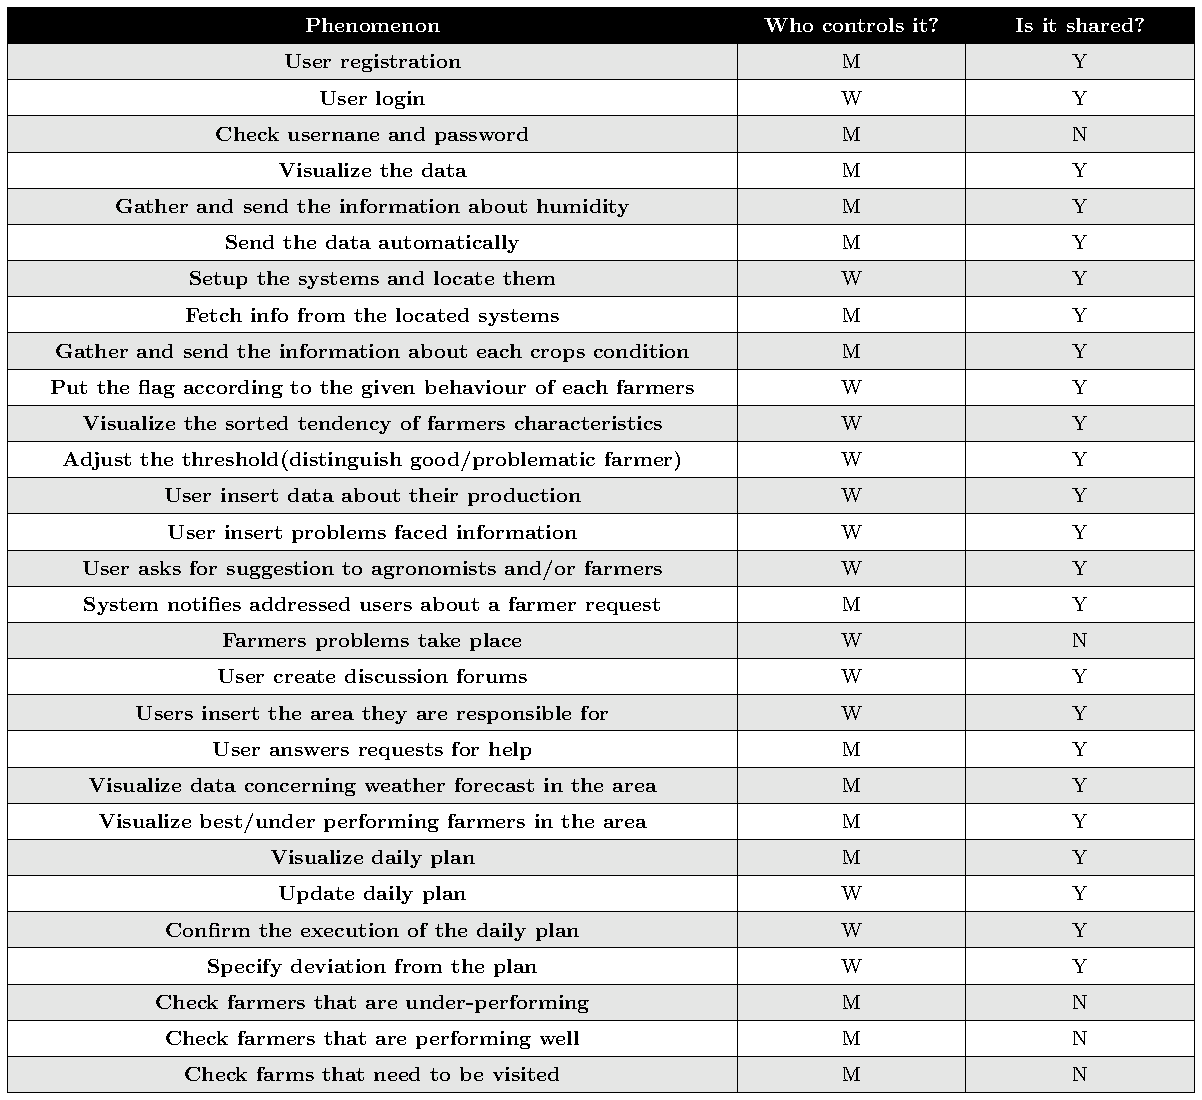
\includegraphics[page=1, width=\textwidth]{Tikz_stuff/Phenomena _table_external_project.pdf}
	\caption{\label{tab:phenomena}Phenomena table}
\end{figure}

% TODO Define verbs conventions of ISO/IEEE
% TODO Requirements should be ranked for importance or stability (from Hans Van Vliet book)

%------------------------------------------------------------------------------------------------------------------------------------------------
\clearpage
{\color{Blue}{\section{Overall Description}}}
\label{sect:overview}

% ############### PRODUCT PERSPECTIVE ####################à
\subsection{Product perspective}
\hyperref[tab:acronymsTable]{DREAM} is a functional multi-user software platform whose purpose is to provide functionalities described in section \ref{sect:product_functions}. The system will be composed by a series of software and hardware interfaces that interact in such a way to let users manipulate shared data. It also will exploit some graphical interface packages in order to be user friendly and easy to use.
This product is designed to run on a wide variety of machines, including operating systems Mac OS, Windows, Linux, Android and iOS. 

\begin{figure}[H]
	\centering
    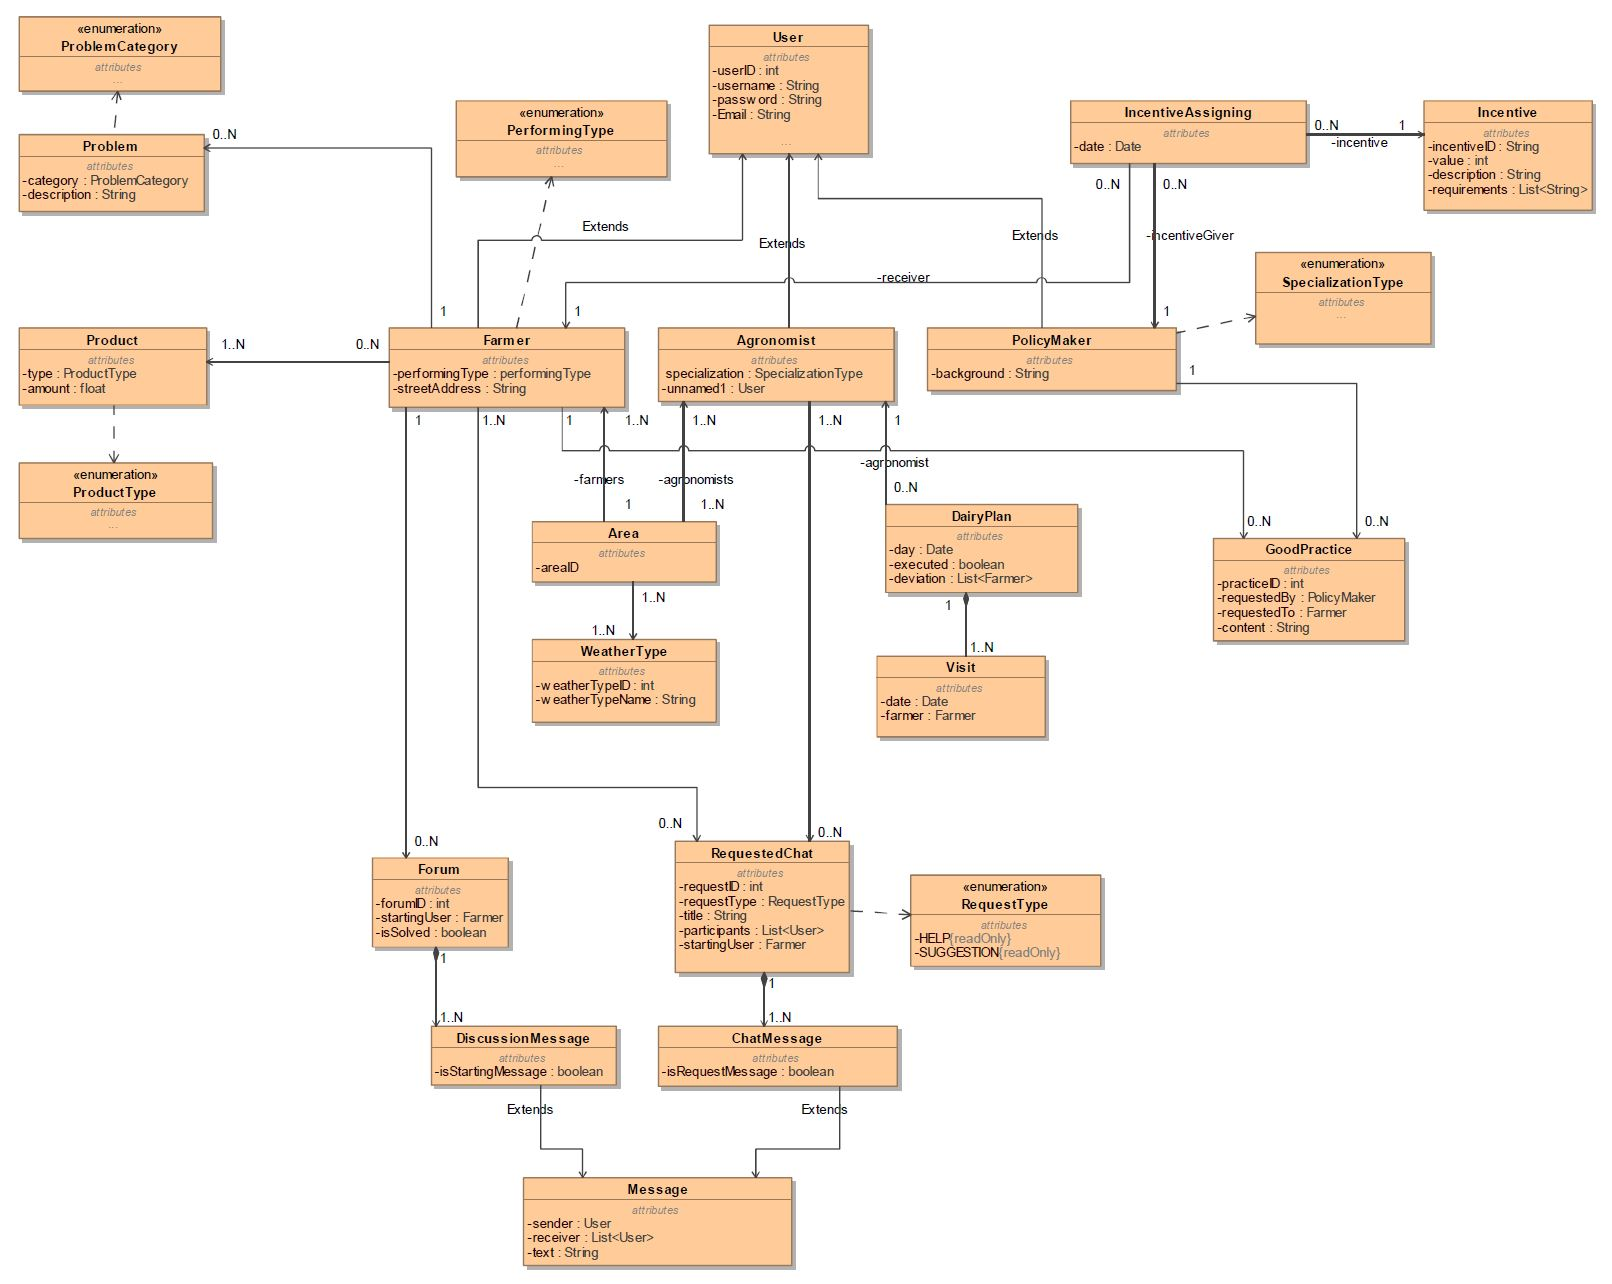
\includegraphics[page=1, width=\textwidth]{Images/uml.JPG}
	\caption{\label{fig:uml_class_diagram}High level UML diagram}
\end{figure}


\subsubsection*{UML description}
\begin{center}
    \setlength\arrayrulewidth{1pt}
    \rowcolors{2}{white}{myblue!25}
    \begin{longtable}{|c|m{0.7\textwidth}|}
            
            \hline
            \rowcolor{myblue}\color{white}Class & \color{white}Description \\
            \hline
            
            \textsc{User}  &    This class represents the people registered to the system, with their credentials  \\
            \hline
            \textsc{Farmer}     &   This class represents the farmers, with their performing type and their street address (information useful to agronomists) \\
            \hline
            \textsc{Agronomist}  &    This class represents the agronomists, with their specialization type \\
            \hline
            \textsc{PolicyMaker}  &    This class represents the policy makers, with their background (e.g., India’s government, Telangana’s government, United Nations, etc)  \\
            \hline
            \textsc{Area}  &    This class represents the areas in which Telangana has been divided for the management of this system. Areas can be the 33 districts in which Telangana is formally divided, but a different subdivision criteria can be used  \\
            \hline
            \textsc{WeatherType}  &    This class represents some characteristics of the area regarding weather aspects (e.g., humidity, rainfall frequency, average temperature, etc)  \\
            \hline
            \textsc{Forum}  &    This class represents the discussion forums that farmers can use to communicate with each other, to get information and to exchange ideas. Only farmers can write in forums  \\
            \hline
            \textsc{RequestChat}  &    This class represents the requests that farmers can send to agronomists and to other farmers. Requests can be for help or for suggestions. A request is modelled as a chat where the participants are selected by the farmer that makes the request. A request always has at least one agronomist as a participant \\
            \hline
            \textsc{Message}  &    This class represents the messages exchanged in forums and chats across the platform, with their sender, receivers and text  \\
            \hline
            \textsc{DiscussionMessage}  &    This class represents the messages belonging to forums. For every forum there is only one starting message, while all the other messages are considered as replies to that message  \\
            \hline
            \textsc{ChatMessage}  &    This class represents the messages belonging to request chats. For every request there is only one message of type “request ”(the first message), while all the other messages are considered as “reply”. Every chat message is delivered to all the participants of that chat (excluding the sender, of course)  \\
            \hline
            \textsc{DailyPlan}  &    This class represents the daily plans of the agronomists, with the date, the list of visits for that day and the list of unvisited farmers (once the plan has been executed)  \\
            \hline
            \textsc{Visit}  &    This class represents the visits that agronomists arrange for checking the farmers’ activity  \\
            \hline
            \textsc{Product}  &    This class represents the products that are inserted in the system by the farmers, with their type and their amount  \\
            \hline
            \textsc{Problem}  &    This class represents the problems that farmers may encounter, with their category and description  \\
            \hline
            \textsc{Incentive}  &    This class represents the incentives that are available for farmers, with their description, their value and their set of requirements. Incentives are modelled as some sort of vouchers  \\
            \hline
            \textsc{IncentiveAssigning}  &    This class represents the assignments of incentives, expressed as a mapping between “when”, “to who” and “from who” a certain incentive has been given  \\
            \hline
            \hline
            \textsc{PerformingType}  &    This enumeration represents the performance type of farmers, giving information about how good a farmer is doing (for example: well-performing, normal-performing, under-performing)  \\
            \hline
            \textsc{SpecializationType}  &    This enumeration represents the type of agronomists’ specializations \\
            \hline
            \textsc{RequestType}  &    This enumeration represents the type of requests, which can be for help or for suggestions  \\
            \hline
            \textsc{ProblemCategory}  &    This enumeration represents the type of problems that farmers can face and insert into the system  \\
            \hline
        
        \rowcolor{white}\caption{UML description table}
        \label{tab:UML_description_table}
    \end{longtable}
\end{center}


\subsubsection{User interfaces}
\label{sect:user_interfaces}
According to the assignment document, the system will interact with 3 different user classes: policy makers, farmers and agronomists. In order to be more accessible and to fulfill the user needs, the application will be supported by different devices. These users should interface to the service through electronic devices with an internet connection. Users that need to access the service will have the possibility to connect through:
\begin{itemize}
    \item an internet browser, addressing a specific web domain (such as \textit{www.dream.com}) that permits users to sign up/in a dedicated web application;
    \item a mobile application that can be installed on smartphones or tablets (both iOS and Android).
\end{itemize}


\subsubsection{Software interfaces}
In order to improve software flexibility and quality, \hyperref[tab:acronymsTable]{DREAM} will use a set of external software interfaces. Rather than providing names of real specific services, we consider reasonable referring to them as functionalities to be later defined in the design phase:
\begin{description}[font=~\normalfont\scshape]
    \item[\textbf{\textcolor{myblue}{universal logins}}] \hfill \\Login \hyperref[tab:acronymsTable]{APIs} that also provide access by using their Facebook, Twitter, or Google profile login details are good candidates in order to quickly authenticate the user while guaranteeing security.
    \item[\textbf{\textcolor{myblue}{big data manipulation}}] \hfill \\Since a wide quantity of information needs to be recorded and accessed in a distributed system fashion, \hyperref[tab:acronymsTable]{DBMS} \hyperref[tab:acronymsTable]{APIs} are necessary for data extraction performances optimization.
    \item[\textbf{\textcolor{myblue}{third party data sets access}}] \hfill \\
    The system will use open data sets to obtain information about weather forecasts, soil moisture, water irrigation, humidity and so on.
    \item[\textbf{\textcolor{myblue}{farmers evaluation}}] \hfill \\
    To evaluate the performance of farmers, the system relies on external \hyperref[tab:acronymsTable]{APIs} that use specific algorithms to understand how good a farmer is doing (positive or negative deviance).
    \item[\textbf{\textcolor{myblue}{incentives management}}] \hfill \\
    The system will rely on an external service for the definition of incentives and for their money collection by the farmers.
    \item[\textbf{\textcolor{myblue}{weather types categorization}}] \hfill \\
    To define the weather type categories of the areas, the system will use some sort of \hyperref[tab:acronymsTable]{API} to analyse areas characteristics and tendencies in order to define shared phenomena. 
    
    
\end{description}

\subsubsection{Hardware interfaces \& constraints}
DREAM system will be composed by multiple different hardware components which can be described from two points of view:
\begin{description}[font=~\normalfont\scshape]
    \item[\textbf{\textcolor{myblue}{user perspective}}] \hfill \\Since \hyperref[tab:acronymsTable]{DREAM} platform is accessed by users in a fully virtual fashion, the minimum required hardware interfaces are the ones that provides internet connection, input components, a screen to visualize \hyperref[tab:acronymsTable]{GUI} and a web browser or an application store (like smartphones, personal computers, tablets and smart TVs).
    \item[\textbf{\textcolor{myblue}{system perspective}}] \hfill \\According to the assignment, the system should be composed by hardware devices designed to gather Telangana's environment information such as soil humidity sensor and the ones responsible for the predefined water irrigation system.
\end{description}
The user hardware interfaces also represent constrains that are required in order to permit the users to interact with the systems and manipulate shared data.

\subsection{Product functions}
\label{sect:product_functions}
In this section the main functionalities of the \hyperref[tab:acronymsTable]{S2B} are presented, described and enriched with \hyperref[tab:acronymsTable]{BPMN} diagrams in order to guarantee an higher level of understanding.
\subsubsection{Sign up}
This functionality allows the user to create an account to access the platform.
Firstly he opens the sign up page and fills the information required such as email, address etc.
Then, if the inserted data is accepted, an e-mail is sent to the User asking for their verification.
Lastly, if all the steps above are done, the user is redirected to the login page.

\begin{figure}[H]
	\centering
    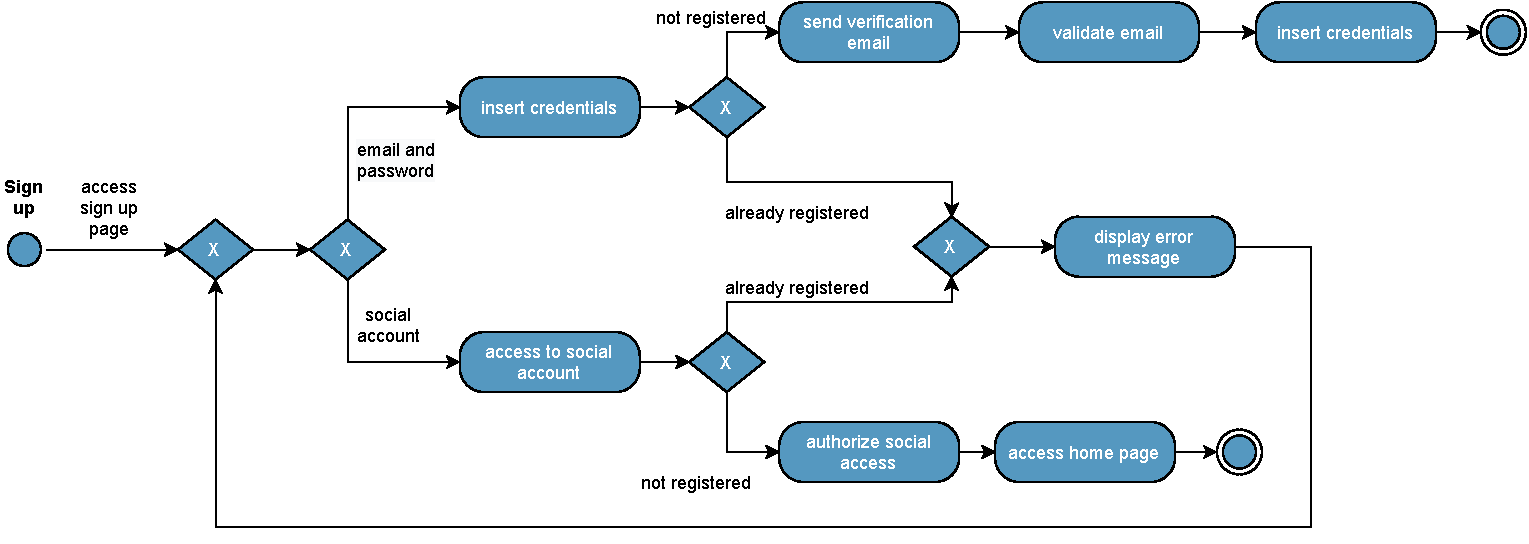
\includegraphics[width=\textwidth]{Images/BPMN/signup.pdf}
	\caption{\label{fig:bpmn_sign_up}BPMN diagram of sign Up}
\end{figure}

\subsubsection{Sharing issues to get help and suggestions}
This functionality is available for farmers and agronomists. The farmer selects the request section and the system displays the send request button; if it is clicked, all the saved contacts are shown. After selecting to whom to ask, insert the question in the text form, presses send button, then the request is sent successfully.


\begin{figure}[H]
	\centering
    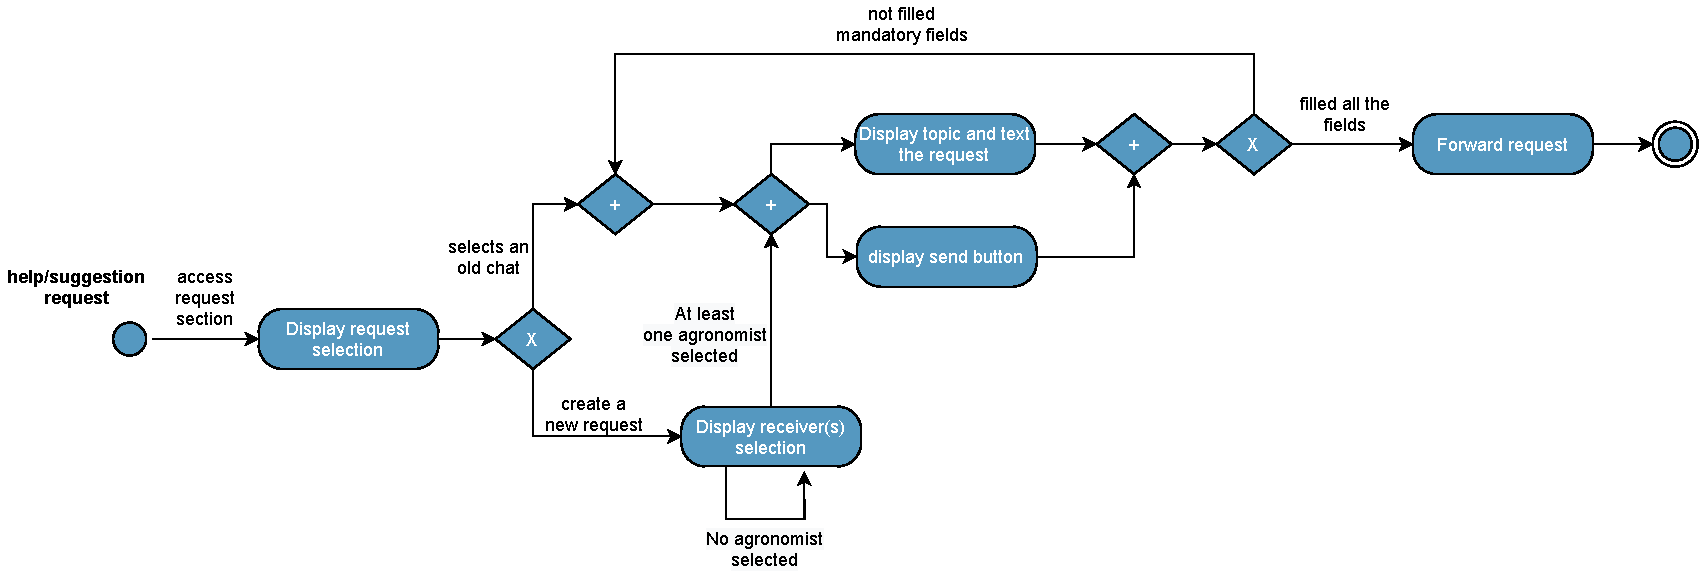
\includegraphics[width=\textwidth]{Images/BPMN/help-suggestion-request.pdf}
	\caption{\label{fig:bpmn_request}BPMN diagram of help/suggestion request}
\end{figure}


\subsubsection{Communication (among farmers) on forums}
This functionality is required for allowing farmers to exchange their opinions. The farmer accesses the forum section which presents an eventual list that contains both previous submitted forums and farmer’s forum replies. By selecting forum upload button, the system displays 
insertion form containing topic/context of the thread, title and question content. If the farmer 
inserts all the required data correctly and presses the submission button, confirmation page is shown. Lastly, by clicking confirm button the forum is generated. 

\begin{figure}[H]
	\centering
    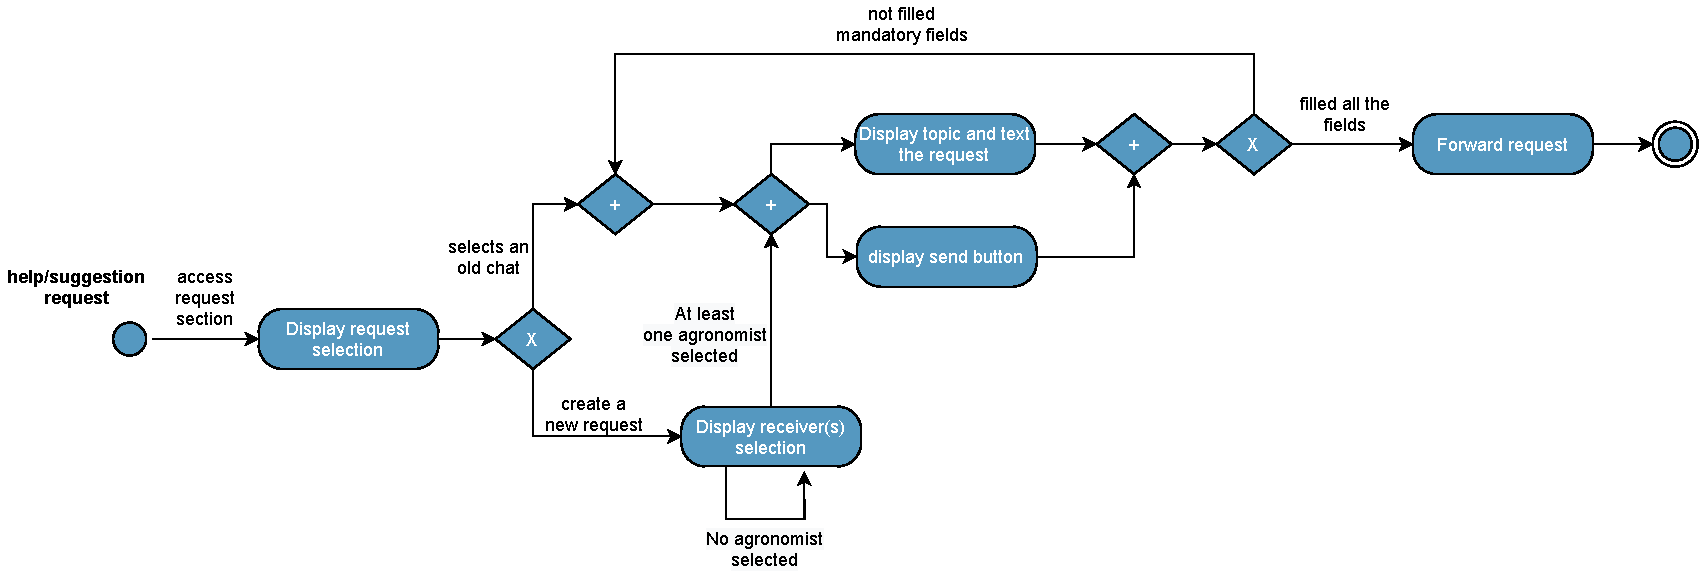
\includegraphics[width=\textwidth]{Images/BPMN/help-suggestion-request.pdf}
	\caption{\label{fig:bpmn_forum_generation}BPMN diagram of forum generation}
\end{figure}


\subsubsection{Visits to low performing farmers}
This functionality is necessary to organize the visits in order to make the schedule well-shared between an agronomist and a farmer. The agronomist goes to the daily plan section and the application displays a visualize or update button. If it is clicked, the system extracts their schedule data which is shortly expressed by a form with day-month-year and the farmers to visit.
If there is a wish to modify the plan, it is possible to modify it in a form guided by selecting the update button.

\begin{figure}[H]
	\centering
    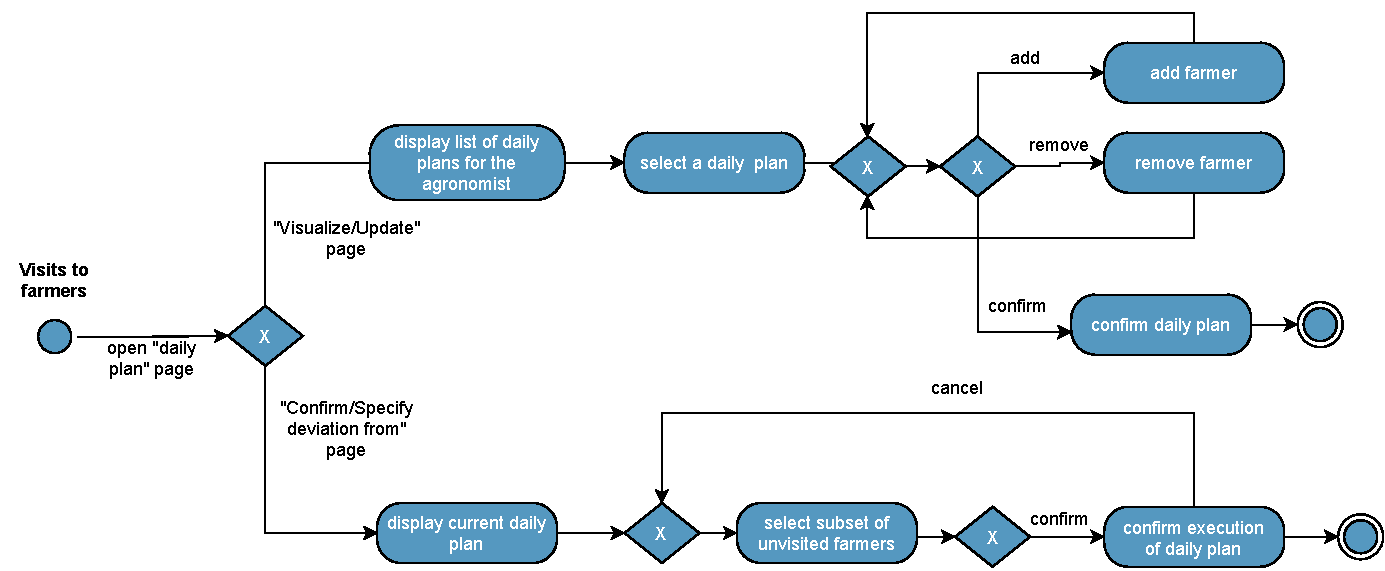
\includegraphics[width=\textwidth]{Images/BPMN/visit.pdf}
	\caption{\label{fig:bpmn_visit}BPMN diagram of visit farmers}
\end{figure}


\subsubsection{Visualize data about performance}
This functionality is used by policy makers. The policy maker clicks the farmer's performance button and the system visualize the list of farmers grouped by their production performance. If there is any interesting farmer, by selecting his/her name, the application shows the information of his/her production history.

\begin{figure}[H]
	\centering
    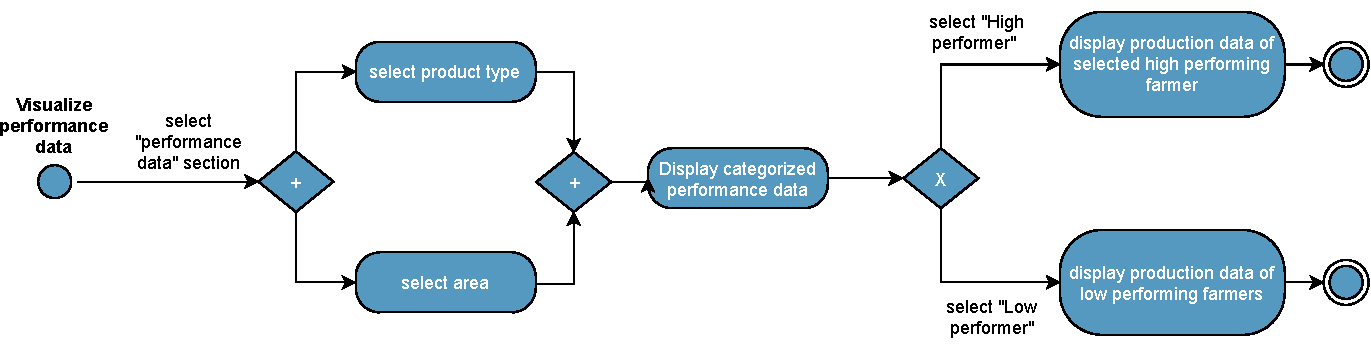
\includegraphics[width=\textwidth]{Images/BPMN/Performance.pdf}
	\caption{\label{fig:bpmn_performance}BPMN diagram of farmer performance}
\end{figure}

\subsection{Actors}
\label{sec:actors}
In this section are defined the professional figures which, according to the assignment, the system will interact with: \textbf{policy makers}, \textbf{farmers} and \textbf{agronomists}. In order to avoid redundancy, we also introduce the concept of \textbf{user} as an abstract entity that collects their common properties. As shown in figure \ref{fig:uml_class_diagram}, they inherit user's properties.
\subsubsection*{User}
It is a person who wants to use the service. In order to access the system, it has to register to the platform (the first time) and be logged in (the following times). It also requires an Internet connection to properly use the system.
\subsubsection*{Policy maker}
It is someone interested in the overall performing situation of Telangana’s farmers (e.g., Telangana’s government). It is able to surf on \hyperref[tab:acronymsTable]{DREAM}’s website. It uses the service to visualise information about well and under-performing farmers and to understand if the steering initiatives are producing significant results. We assume that those who register to the platform as policy makers are some sort of "authorized" people (for example, people working for public institutions or government) since they are allowed to actively assign incentives.
\subsubsection*{Farmer}
It is a farmer of Telangana. It is able to surf on \hyperref[tab:acronymsTable]{DREAM}’s website (or to use the smartphone application). It uses the service in order to discuss with other farmers, to send requests for help to an agronomist, to insert product information, to know when it will receive a visit from an agronomist. It takes advantage in using the system because it can receive incentives if it is well-performing or can receive help if it is under-performing.
\subsubsection*{Agronomist}
It is an agronomist of Telangana. It is able to surf on \hyperref[tab:acronymsTable]{DREAM}’s website (or to use the smartphone application). It uses the service to answer farmers' requests for help, to visualise data concerning their areas (weather forecasts, well and under-performing farmers, problems encountered by farmers), to visualise and update a daily plan to visit farms in the area, to confirm the execution or specify deviation from the daily plan.

\newpage

\subsection{Assumptions, dependencies and constraints}
\label{sec:domain_assumptions}
In this section we present the assumptions that are expected to hold in the world, the part of the environment that the machine cannot perceive nor control. The satisfaction of these so called \textbf{domain assumptions} are deeply related to the reliability of the system to behave in the expected way. If at least one of these assumptions is discovered not to be guaranteed, then the expected behaviour of the machine would allow the occurrence of an unstable state of the machine with unpredictable results.
\newline

\begin{table}[H]
    \setlength\arrayrulewidth{1pt}
    \centering
    \rowcolors{2}{white}{myblue!25}
    \begin{tabular}{|l|m{0.85\textwidth}|}
        \rowcolor{myblue}
        \hline
        \color{white}DX & \color{white}Definition \\
        \hline
        \textsc{D1}  &    Data concerning meteorological short-term and long-term forecasts is exact and reliable \\
        \hline
        \textsc{D2}     &   Information obtained by the water irrigation system is reliable \\
        \hline
        \textsc{D3}  &    Information on the humidity of soil obtained by sensors deployed on the territory is reliable\\
        \hline
        \textsc{D4}  &    Each user who wants to use the online service (web page, app) must have a device connected to Internet\\
        \hline
        \textsc{D5}  &    The user is supposed to be at least 18 years old\\
        \hline
        \textsc{D6}  &    The third party analysis about how good a farmer is doing is reliable\\
        \hline
        \textsc{D7}  &    The categorized weather types provided by a third party analysis are reliable\\
        \hline
        \textsc{D8}  &     The weather information provided by a third party is reliable \\
        \textsc{D9}  &     The third party analysis about the effectiveness of the steering initiatives is reliable \\
        \hline
        
        \hline
        \hline
        \hline
        \textsc{D10}  &    Observation of  farmers' performance is done frequently by policy makers\\
        \hline
        \textsc{D11}  &    Policy maker has enough information and knowledge to understand the proper moment to ask for good practices\\
        \hline
        \textsc{D12}  &    Outstanding high performing farmers are asked by policy makers to write their good practices periodically\\
        \hline
        \textsc{D13}  &     Incentive assignment done by policy makers is reliable \\
        \hline
        
        \hline
        \hline
        \hline
        
        \textsc{D14}  &    Information stored in the system by farmers is reliable (e.g. farmers do not insert false data about their production or their problems to look better/worse performing)\\
        \hline
        \textsc{D15}  &    When a problem occurs, farmers insert that information in the system\\
        \hline
        \textsc{D16}  &    Farmers usually interact with the system (periodic product information upload, checking for agronomist visits) \\
        \hline
        \textsc{D17}     &   When a farmer starts a forum thread, a reply will be given as soon as possible \\
        \hline
        \textsc{D18}  &    Farmer agrees on allowing the system to store information about them (location of the activity, information on production, ...)\\
        \hline
        
        
        \hline
        \hline
        \hline
    
        \textsc{D19}  &    Information inserted in the system by agronomists is reliable\\
        \hline
        \textsc{D20}  &    When an agronomist plans the visits of a daily plan, most farmers will be present\\
        \hline
        \textsc{D21}  &    Agronomists will always confirm the execution (specifying deviations, if needed) of the daily plan at the end of the same day\\
        \hline
        \textsc{D22}  &    An agronomist is responsible for several areas\\
        \hline
        
        
        
       
        
        
    \end{tabular}
    
    \caption{\label{tab:domainAssumptions}Table of domain assumptions}
    
\end{table}

\tmref{link to traceability matrix}

%------------------------------------------------------------------------------------------------------------------------------------------------
\clearpage
{\color{Blue}{\section{Specific Requirements}}}
\label{sect:requirements}
In this chapter there will be defined \ldots


\subsection{External Interface Requirements}
\subsubsection{User Interfaces}
\subsubsection{Hardware Interfaces}
\subsubsection{Software Interfaces}
\subsubsection{Communication Interfaces}


\subsection{Functional Requirements}
\subsubsection{User scenarios}
\subsubsection{Policy maker scenarios}
\subsubsection{Farmer scenarios}
\subsubsection{Agronomist scenarios}
\subsubsection{Requirements}
\subsubsection{Traceability Matrix}

\subsection{Performance Requirements}


\subsubsection{Policy makers}
\label{sect:policy_maker_requirements}
% Moved to section 1.4 Definitions, acronyms, abbreviations


\begin{table}[H]
    \centering
    \begin{tabular}{|l|p{0.75\textwidth}|}
        \hline % ---------------------------------------------------------------------
    	\textsc{id}                 &   PM.1\\
    	\hline % ---------------------------------------------------------------------
    	\textsc{Name}               &   Visualize the performance data of each farmer\\
    	\hline % ---------------------------------------------------------------------
    	\textsc{Actor}             &   Policy maker\\
    	\hline % ---------------------------------------------------------------------
    	\textsc{Entry condition}   &   Policy maker has logged in\\
    	\hline % ---------------------------------------------------------------------
    	\textsc{Events flow}         &   %\footnotesize
            	                        \begin{itemize}
                                    	    \item Policy maker presses the button “Farmer’s performance”
                                    	    \item The system displays options to let user select filters about weather type, product type
                                    		\item Policy maker selects desired filters
                                    		\item The system displays the list of farmers divided by performance
                                    		\item Policy maker selects interested farmer’s name
                                    		\item The system shows detailed information about that farmer’s production
                                        \end{itemize}\\
        \hline % ---------------------------------------------------------------------
        \textsc{Exit condition}    &  The system returns to the main page of policy maker\\
    	\hline % ---------------------------------------------------------------------
    	\textsc{Output}             &  \begin{itemize}
    	    \item Policy maker has obtained the farmer's production data they were looking for
    	\end{itemize}\\
    	\hline % ---------------------------------------------------------------------
    	\textsc{Exception}         &  Policy maker could not find the name of farmer who should exist. The system displays the error message\\
    	\hline % ---------------------------------------------------------------------
        
    \end{tabular}
    \caption{\label{tab:visualize_farmer_performance}Visualize the performance data of farmers} 
\end{table}

\begin{figure}[H]
    \centering
    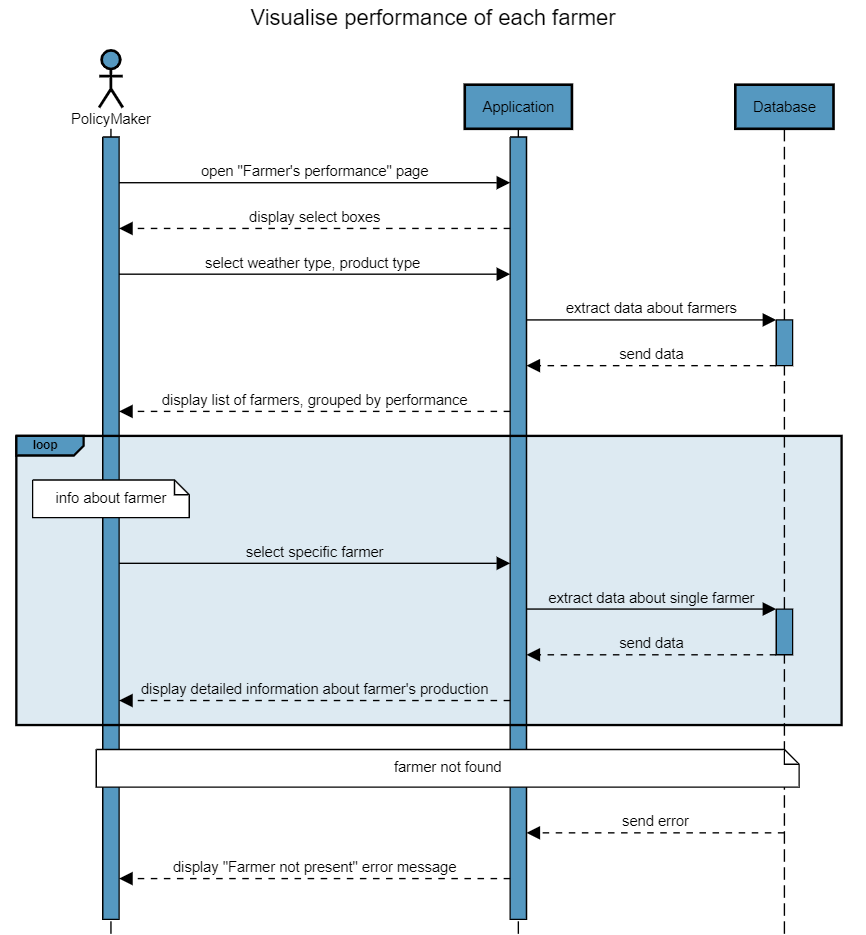
\includegraphics[scale=0.5]{Images/Sequence diagrams/SE2 - visualize performance (pm).png}
    \caption{Visualize the performance data of farmers - sequence diagram}
    \label{fig:my_label}
\end{figure}

\begin{table}[H]
    \centering
    \begin{tabular}{|l|p{0.75\textwidth}|}
        \hline % ---------------------------------------------------------------------
    	\textsc{id}                 &   PM.2\\
    	\hline % ---------------------------------------------------------------------
    	\textsc{Name}               &   Manage the incentives of high performing farmers \\
    	\hline % ---------------------------------------------------------------------
    	\textsc{Actor}             &   Policy maker\\
    	\hline % ---------------------------------------------------------------------
    	\textsc{Entry condition}   &   Policy maker has logged in\\
    	\hline % ---------------------------------------------------------------------
    	\textsc{Events flow}         &   %\footnotesize
            	                        \begin{itemize}
                                    	    \item Policy maker presses the button “Farmer’s performance”
                                    		\item The system displays a page with the list of farmers (grouped by performance) and a column which clarifies the status of their incentives 
                                       		\item Policy maker selects the interested farmer’s incentive column
                                    		\item The system shows detailed information about farmer’s incentives status
                                    		\item Policy maker clicks "Select incentive" button
                                    		\item The system shows the possible choices
                                    		\item Policy maker selects the incentive to give
                                    		\item The system shows the popup to ask a confirmation to proceed
                                    		\item Policy maker clicks "Confirm" button
                                    		\item The system shows the updated incentive column
                                        \end{itemize}\\
        \hline % ---------------------------------------------------------------------
        \textsc{Exit condition}    &  The system returns to the main page of policy maker\\
    	\hline % ---------------------------------------------------------------------
    	\textsc{Output}             &  \begin{itemize}
    	    \item Policy maker has managed the incentive to give
    	    \item The farmer correctly received the inventive
    	\end{itemize}\\
    	\hline % ---------------------------------------------------------------------
    	\textsc{Exception}         &  Policy maker wrongly selects an incentive data. The 
    	system shows a popup to ask a confirmation to proceed. The policy maker can redo the operation by clicking on “Cancel” button\\
    	\hline % ---------------------------------------------------------------------
        
    \end{tabular}
    \caption{\label{tab:visualize_incentives}Manage the incentives of farmers} 
\end{table}

\begin{figure}[H]
    \centering
    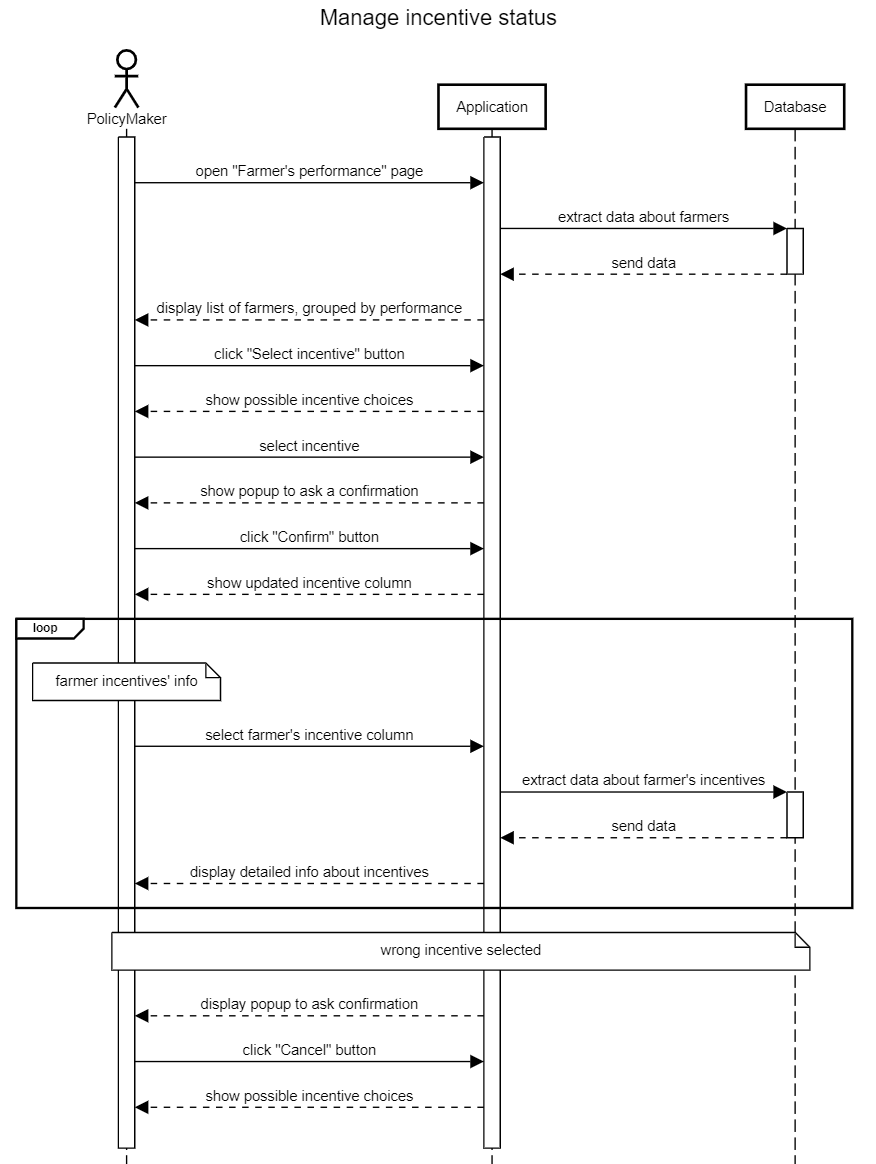
\includegraphics[scale=0.5]{Images/Sequence diagrams/SE2 - manage incentive status (pm).png}
    \caption{Manage the incentives of farmers - sequence diagram}
    \label{fig:my_label}
\end{figure}

\begin{table}[H]
    \centering
    \begin{tabular}{|l|p{0.75\textwidth}|}
        \hline % ---------------------------------------------------------------------
    	\textsc{id}                 &   PM.3\\
    	\hline % ---------------------------------------------------------------------
    	\textsc{Name}               &   Visualize the effectiveness of the steering initiatives\\
    	\hline % ---------------------------------------------------------------------
    	\textsc{Actor}             &   Policy maker\\
    	\hline % ---------------------------------------------------------------------
    	\textsc{Entry condition}   &   Policy maker has logged in\\
    	\hline % ---------------------------------------------------------------------
    	\textsc{Events flow}         &   %\footnotesize
            	                        \begin{itemize}
                                    	    \item Policy maker presses the button “Effectiveness of initiatives”
                                    	    \item The system displays options to let user select filters about weather type, product type
                                    		\item Policy maker selects the desired filters
                                    		\item The system displays a page with categorized farmers, highlighting those who have improved their performance significantly within a year
                                    		\item Policy maker selects interested farmer’s name
                                    		\item The system shows detailed information about the farmer’s performance trend, the problems encountered, the history of requests and visits
                                        \end{itemize}\\
        \hline % ---------------------------------------------------------------------
        \textsc{Exit conditions}    &  The system returns to the main page of policy maker\\
    	\hline % ---------------------------------------------------------------------
    	\textsc{Output}             &  \begin{itemize}
    	    \item Policy maker has obtained the history of performance data and interaction between farmers and agronomists they were looking for
    	\end{itemize}\\
    	\hline % ---------------------------------------------------------------------
    	\textsc{Exception}         &  Policy maker couldn’t find the name of farmer who should exist. The system displays the error message\\
    	\hline % ---------------------------------------------------------------------
        
    \end{tabular}
    \caption{\label{tab:visualize_iprovement}Visualize the effectiveness of the steering initiatives}
\end{table}

\begin{figure}[H]
    \centering
    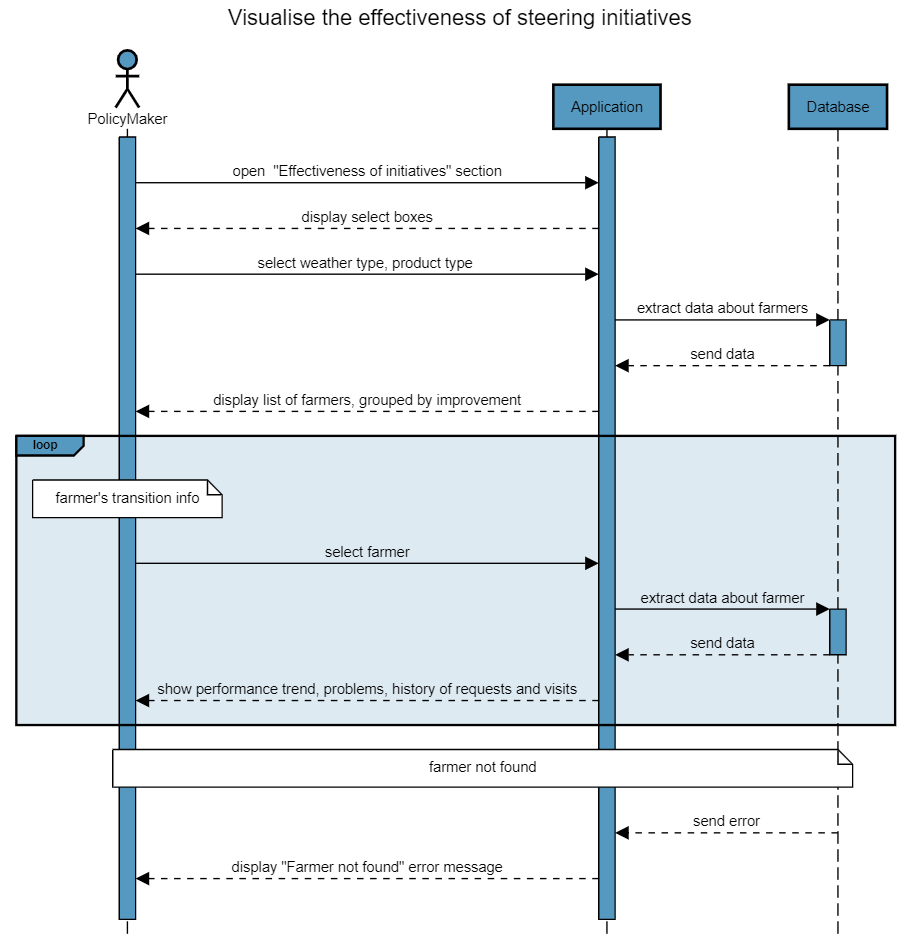
\includegraphics[scale=0.5]{Images/Sequence diagrams/SE2 - visualise effectiveness of steering initiatives (pm).png}
    \caption{Visualize the effectiveness of the steering initiatives - sequence diagram}
    \label{fig:my_label}
\end{figure}

\begin{table}[H]
    \centering
    \begin{tabular}{|l|p{0.75\textwidth}|}
        \hline % ---------------------------------------------------------------------
    	\textsc{id}                 &   PM.4\\
    	\hline % ---------------------------------------------------------------------
    	\textsc{Name}               &   Ask high performing farmers to write good practices\\
    	\hline % ---------------------------------------------------------------------
    	\textsc{Actor}             &   Policy maker\\
    	\hline % ---------------------------------------------------------------------
    	\textsc{Entry condition}   &   Policy maker has logged in\\
    	\hline % ---------------------------------------------------------------------
    	\textsc{Events flow}         &   %\footnotesize
            	                        \begin{itemize}
                                    	    \item Policy maker presses the button “Farmer’s performance”
                                    		\item The system displays a page with the list of farmers grouped by performance
                                    		\item Policy maker selects interested high performing farmer’s name
                                    		\item The system shows the detailed information about farmer’s production and "request writing" button
                                    		\item Policy maker clicks "equest writing" button
                                    		\item The system shows a popup to ask the confirmation to proceed
                                    		\item Policy maker clicks "Confirm" button
                                    		\item The system sends the request to the selected farmer and shows a message to notify the success of the operation
                                        \end{itemize}\\
        \hline % ---------------------------------------------------------------------
        \textsc{Exit condition}    &  The system returns to the Farmer’s performance page\\
    	\hline % ---------------------------------------------------------------------
    	\textsc{Output}             &  \begin{itemize}
    	    \item Policy maker has requested the high performing farmer to write their good practice
    	\end{itemize}\\
    	\hline % ---------------------------------------------------------------------
    	\textsc{Exception}         &  Policy maker wrongly selects a farmer. The 
    	system shows a popup to ask a confirmation to proceed. The policy maker can redo the operation by clicking on “Cancel” button\\
    	\hline % ---------------------------------------------------------------------
        
    \end{tabular}
    \caption{\label{tab:visualize_iprovement}Ask a farmer to write good practices} 
\end{table}

\begin{figure}[H]
    \centering
    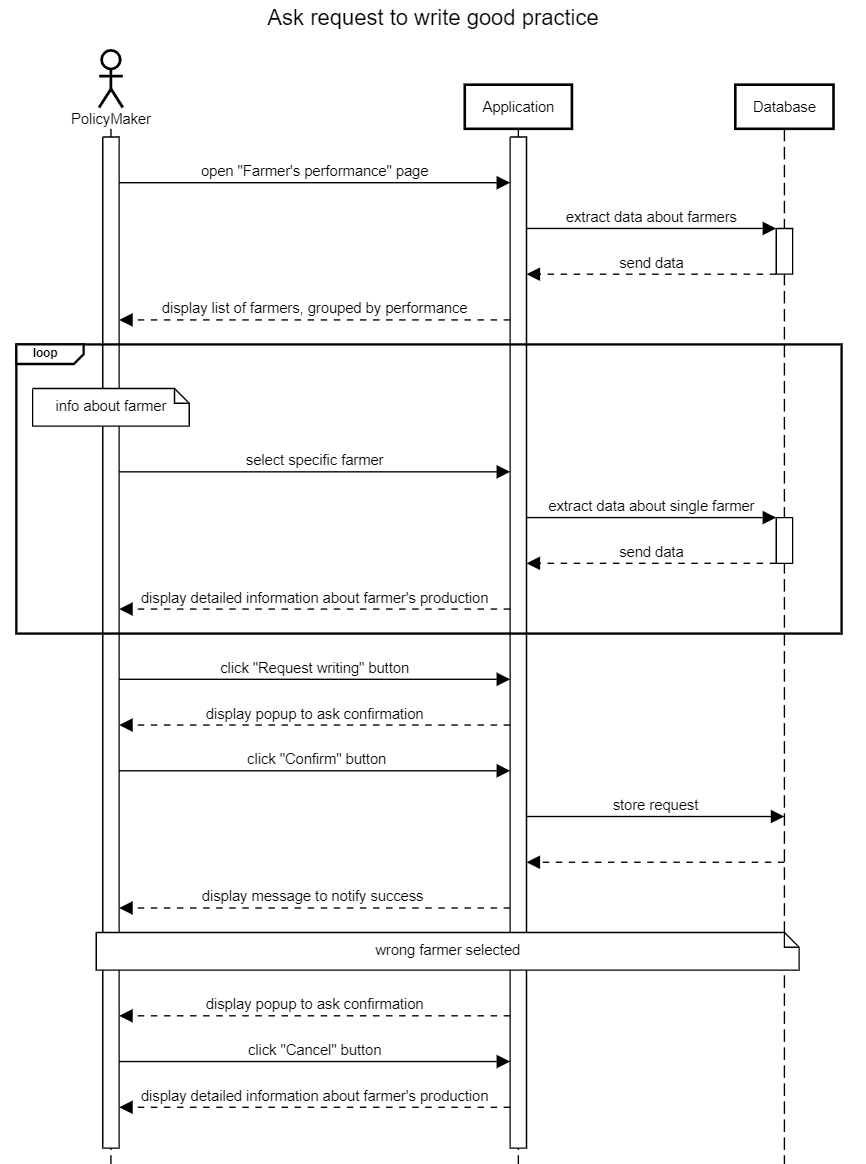
\includegraphics[scale=0.5]{Images/Sequence diagrams/SE2 - Ask request to write good practice (pm).png}
    \caption{Ask request to write good practice - sequence diagram}
    \label{fig:my_label}
\end{figure}


\subsubsection{Farmers}
\label{sect:farmer_requirements}
Synonims: system, application, service


% ####################### 1 PRODUCTION DATA UPLOAD ###################

\begin{table}[H]
    \centering
    \begin{tabular}[c]{|l|p{0.75\textwidth}|}
        \hline % ---------------------------------------------------------------------
    	\textsc{id}                 &   F.1\\
    	\hline % ---------------------------------------------------------------------
    	\textsc{Name}               &   Production data upload\\
    	\hline % ---------------------------------------------------------------------
    	\textsc{Actor}             &   Farmer\\
    	\hline % ---------------------------------------------------------------------
    	\textsc{Entry condition}   &   Farmer has logged in\\
    	\hline % ---------------------------------------------------------------------
    	\textsc{Events flow}         &   %\footnotesize
            	                        \begin{itemize}
                                    	    \item Farmer goes to the \textit{Record Production Data} section
                                    		\item The application displays a section that asks for \hyperref[tab:definitionsTable]{product information} and an \textit{Upload Button}
                                    		\item Farmer fills the mandatory fields of the current section and eventually the optional ones. Then press the \textit{Upload Button}.
                                    		\item The application displays a confirm popup revealing the summary of the information is going to be recorded, asking for Farmer confirmation through a \textit{Confirm Button}
                                    		\item The farmer confirms the submission by selecting the Confirm Button
                                        \end{itemize}\\
        \hline % ---------------------------------------------------------------------
        \textsc{Exit condition}    &  The application displays the summary page of both already uploaded product information and the previous submitted ones\\
    	\hline % ---------------------------------------------------------------------
    	\textsc{Output}             &  \begin{itemize}
    	    \item The system collects the new production data
    	    \item The farmer can visualize the list of both current production information and the previous ones
    	\end{itemize}\\
    	\hline % ---------------------------------------------------------------------
    	\textsc{Exception}         &  Farmer submits production data without filling the mandatory fields. In such case, the system displays an error message informing the Farmer about the missing field(s) required in order to achieve the goal\\
    	\hline % ---------------------------------------------------------------------
        
    \end{tabular}
    \caption{\label{tab:Production_data_submission}Production data upload}
\end{table}


\begin{figure}[H]
	\centering
    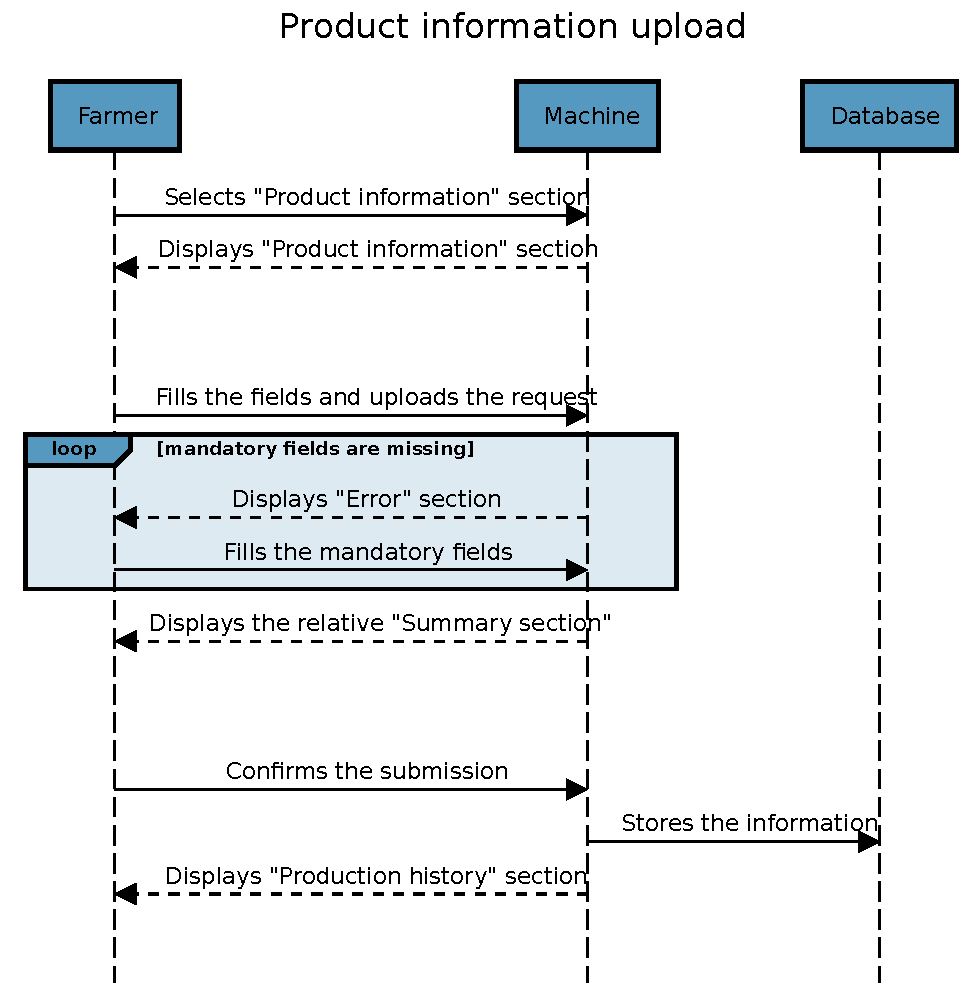
\includegraphics[page=1, width=\textwidth]{Images/SeqDiag/product_info_upload_seq_diag.pdf}
	\caption{\label{fig:product_info_seq_diag}Production data upload - sequence diagram}
\end{figure}


% ####################### 2 SUGGESTION REQUEST ###################

\begin{table}[H]
    \centering
    \begin{tabular}{|l|p{0.75\textwidth}|}
        \hline % ---------------------------------------------------------------------
    	\textsc{id}                 &   F.2\\
    	\hline % ---------------------------------------------------------------------
    	\textsc{Name}               &   Help/suggestion request\\
    	\hline % ---------------------------------------------------------------------
    	\textsc{Actor}             &   Farmer\\
    	\hline % ---------------------------------------------------------------------
    	\textsc{Entry condition}   &   Farmer has logged in\\
    	\hline % ---------------------------------------------------------------------
    	\textsc{Events flow}         &   %\footnotesize
            	                        \begin{itemize}
                                    	    \item Farmer selects the graphical section responsible of the private requests, called informally \textit{request section} for the sake of simplicity
                                    		\item The application displays a section that presents an eventual list of previous request chats and an additional button to send a new private request, called informally \textit{Send request element}
                                    		\item Farmer clicks on the send request button
                                    		\item The application displays a new section asking for the selection of the receivers
                                    		\item The farmer selects the contact he wants to send the request
                                    		\item The system displays a section with an editable text form, asks for the selection of the topic of the request and displays a send button
                                    		\item The farmer writes the request, fills the topic form and clicks on the send button
                                        \end{itemize}\\
        \hline % ---------------------------------------------------------------------
        \textsc{Exit condition}    &  The application displays the summary page of both already sent request chat and the previous submitted ones\\
    	\hline % ---------------------------------------------------------------------
    	\textsc{Output}             &  \begin{itemize}
    	    \item The system collects the new request chat
    	    \item The farmer can visualize the list of both current request chat and the previous ones
    	\end{itemize}\\
    	\hline % ---------------------------------------------------------------------
    	\textsc{Exception}         &  Farmer clicks on the request button without editing the text form. In such case, the system displays an error message informing the Farmer about the missing field required in order to achieve the goal\\
    	\hline % ---------------------------------------------------------------------
        
    \end{tabular}
    \caption{\label{tab:Help_request_submission}Help/suggestion request}

\end{table}

\begin{figure}[H]
	\centering
    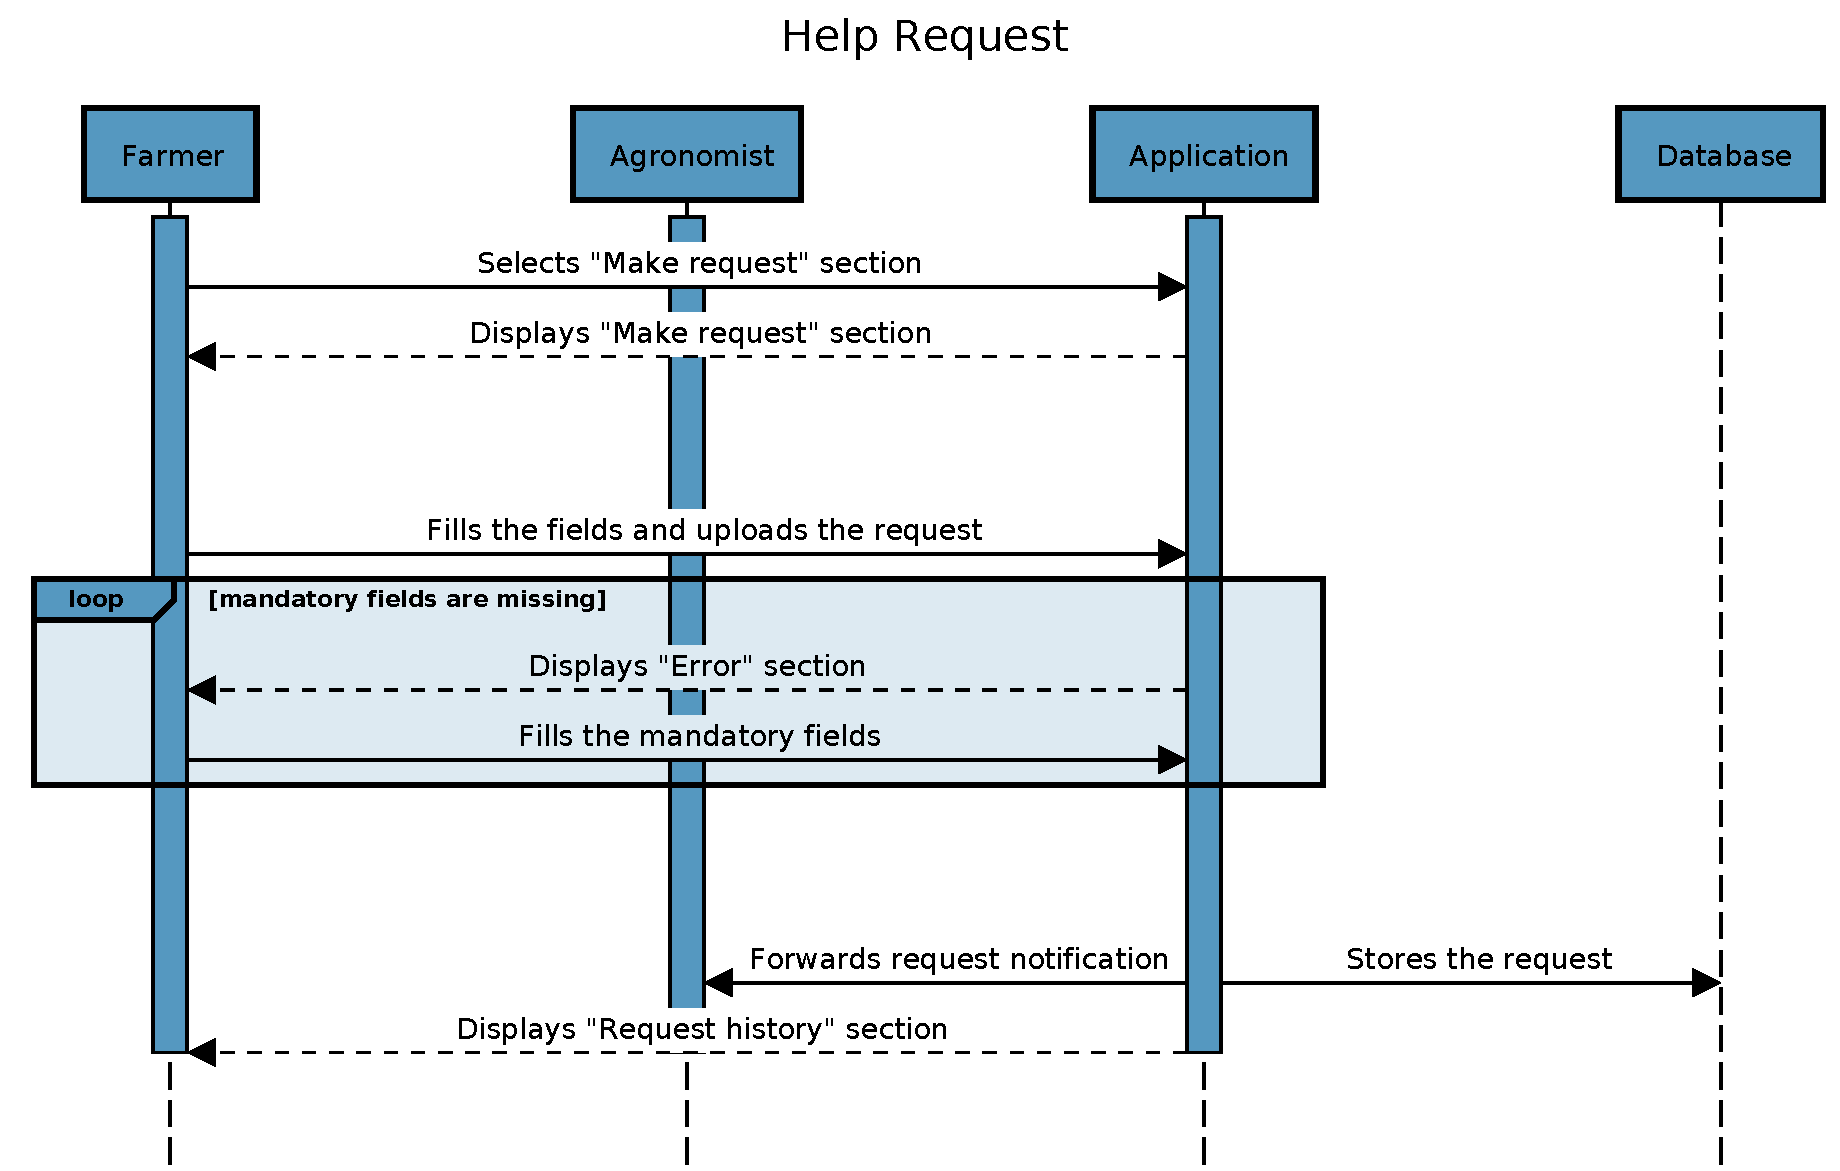
\includegraphics[page=1, width=\textwidth]{Images/SeqDiag/help_request_seq_diag.pdf}
	\caption{\label{fig:help_request_seq_diag}Help request - sequence diagram}
\end{figure}

% ####################### 3 FORUM GENERATION ###################

\begin{table}[H]
    \centering
    \begin{tabular}{|l|p{0.75\textwidth}|}
        \hline % ---------------------------------------------------------------------
    	\textsc{id}                 &   F.3\\
    	\hline % ---------------------------------------------------------------------
    	\textsc{Name}               &   Forum generation\\
    	\hline % ---------------------------------------------------------------------
    	\textsc{Actor}             &   Farmer\\
    	\hline % ---------------------------------------------------------------------
    	\textsc{Entry condition}   &   Farmer has logged in\\
    	\hline % ---------------------------------------------------------------------
    	\textsc{Events flow}         &   %\footnotesize
            	                        \begin{itemize}
                                    	    \item Farmer selects the graphical section responsible of the forum generation, called informally \textit{Forum section} for the sake of simplicity
                                    		\item The application displays a section that presents an eventual list that contains both previous submitted forums and the ones farmer replied, and an internal element to submit a new public forum, called informally \textit{forum upload button}
                                    		\item Farmer selects the forum upload button
                                    		\item The application displays a new section that present 3 mandatory fields (the topic/context of the thread, the title and the question content) and a submission button
                                    		\item The farmer fills all the mandatory fields and selects the submission button
                                    		\item The application displays a confirm popup revealing the summary of the information is going to be uploaded, asking for Farmer confirmation through a \textit{Confirm Button}
                                    		\item The farmer confirms the submission by selecting the Confirm Button
                                        \end{itemize}\\
        \hline % ---------------------------------------------------------------------
        \textsc{Exit condition}    &  The application displays the summary page containing both already submitted forum thread, the previous submitted ones and the ones to which the farmer replied\\
    	\hline % ---------------------------------------------------------------------
    	\textsc{Output}             &  \begin{itemize}
    	    \item The system collects the new forum thread
    	    \item The farmer can visualize the list containing both current forum thread, the previous submitted ones and the ones whose the farmer replied
    	\end{itemize}\\
    	\hline % ---------------------------------------------------------------------
    	\textsc{Exception}         &   Farmer submits Forum thread without filling all the mandatory fields. In such case, the system displays an error message informing the Farmer about the missing field(s) required in order to achieve the goal\\
    	\hline % ---------------------------------------------------------------------
        
    \end{tabular}


    \caption{\label{tab:Forum_generation}Forum generation}
\end{table}

\begin{figure}[H]
	\centering
    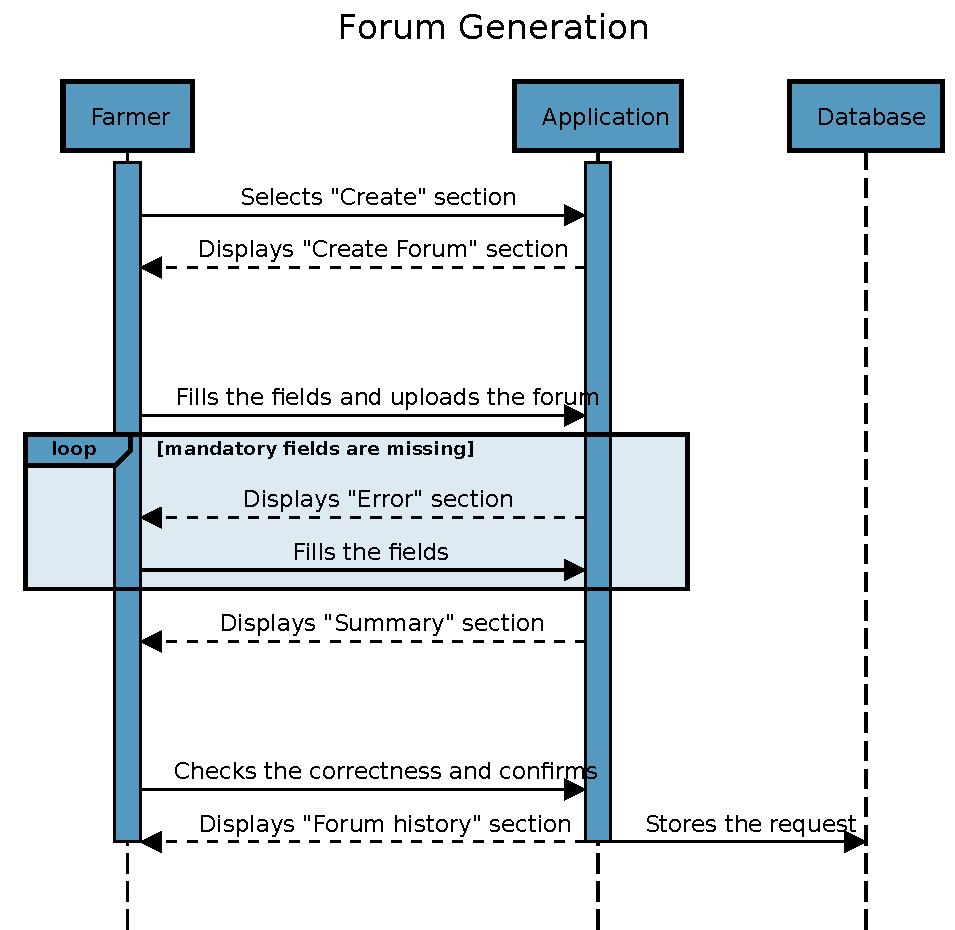
\includegraphics[page=1, width=\textwidth]{Images/SeqDiag/forum_generation_seq_diag.pdf}
	\caption{\label{fig:forum_generation_seq_diag}Forum generation - sequence diagram}
\end{figure}

% ####################### 4 PROBLEM INFORMATION ###################


\begin{table}[H]
    \centering
    \begin{tabular}{|l|p{0.75\textwidth}|}
        \hline % ---------------------------------------------------------------------
    	\textsc{id}                 &   F.4\\
    	\hline % ---------------------------------------------------------------------
    	\textsc{Name}               &   Problem information upload\\
    	\hline % ---------------------------------------------------------------------
    	\textsc{Actor}             &   Farmer\\
    	\hline % ---------------------------------------------------------------------
    	\textsc{Entry condition}   &   Farmer has logged in\\
    	\hline % ---------------------------------------------------------------------
    	\textsc{Events flow}         &   %\footnotesize
            	                        \begin{itemize}
                                    	    \item Farmer selects the graphical section responsible for the problem information submission, called informally \textit{Problems section}
                                    		\item The application displays a section that requires for information (described previously) and a "submit button"
                                    		\item Farmer fills the mandatory fields and eventually the optional ones, then selects the upload button
                                    		\item The application displays a confirm popup revealing the summary of the information is going to be uploaded, asking for Farmer confirmation through a \textit{Confirm Button}
                                    		\item The farmer confirms the submission by selecting the Confirm Button
                                        \end{itemize}\\
        \hline % ---------------------------------------------------------------------
        \textsc{Exit condition}    &  The application displays the summary page containing both already submitted problem information and the previous submitted ones\\
    	\hline % ---------------------------------------------------------------------
    	\textsc{Output}             &  \begin{itemize}
    	    \item The system collects the new problem information instance
    	    \item The farmer can visualize the list containing both the current submitted problem information and the previous submitted ones
    	\end{itemize}\\
    	\hline % ---------------------------------------------------------------------
    	\textsc{Exception}         &   Farmer submits problem information without filling all the mandatory fields. In such case, the system displays an error message informing the Farmer about the missing field(s) required in order to achieve the goal\\
    	\hline % ---------------------------------------------------------------------
        
    \end{tabular}

\caption{\label{tab:problem_information}Problem information upload}
\end{table}

\begin{figure}[H]
	\centering
    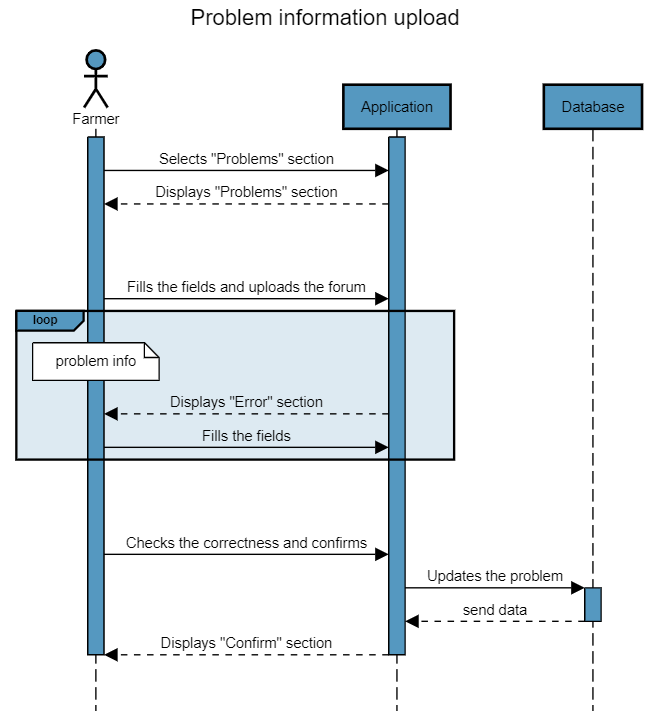
\includegraphics[page=1, width=\textwidth]{Images/Sequence diagrams/SW2- Problem information upload (fa).png}
	\caption{\label{fig:good_practice_seq_diag}Problem information upload - sequence diagram}
\end{figure}

% ####################### 5 GOOD PRACTICES ###################

\begin{table}[H]
    \centering
    \begin{tabular}{|l|p{0.75\textwidth}|}
        \hline % ---------------------------------------------------------------------
    	\textsc{id}                 &   F.5\\
    	\hline % ---------------------------------------------------------------------
    	\textsc{Name}               &   Good practices upload\\
    	\hline % ---------------------------------------------------------------------
    	\textsc{Actor}             &   Farmer\\
    	\hline % ---------------------------------------------------------------------
    	\textsc{Entry condition}   &   Farmer has logged in\\
    	\hline % ---------------------------------------------------------------------
    	\textsc{Events flow}         &   %\footnotesize
            	                        \begin{itemize}
                                    	    \item Farmer selects the graphical section responsible for the good practices document submission, called informally \textit{document section}
                                    		\item The application displays a section that requires for information (described previously) and a "submit button"
                                    		\item Farmer fills the mandatory fields and eventually the optional ones, then selects the upload button
                                    		\item The farmer confirms the submission by selecting the Confirm Button
                                        \end{itemize}\\
        \hline % ---------------------------------------------------------------------
        \textsc{Exit condition}    &  The application displays the summary page containing both already submitted document and the previous submitted ones\\
    	\hline % ---------------------------------------------------------------------
    	\textsc{Output}             &  \begin{itemize}
    	    \item The system collects the new document
    	    \item The farmer can visualize the list containing both the current submitted document and the previous submitted ones
    	\end{itemize}\\
    	\hline % ---------------------------------------------------------------------
    	\textsc{Exception}         &   Farmer submits document without filling all the mandatory fields. In such case, the system displays an error message informing the Farmer about the missing field(s) required in order to achieve the goal\\
    	\hline % ---------------------------------------------------------------------
        
    \end{tabular}

\caption{\label{tab:good_practice_submission}Good practices upload}
\end{table}

\begin{figure}[H]
	\centering
    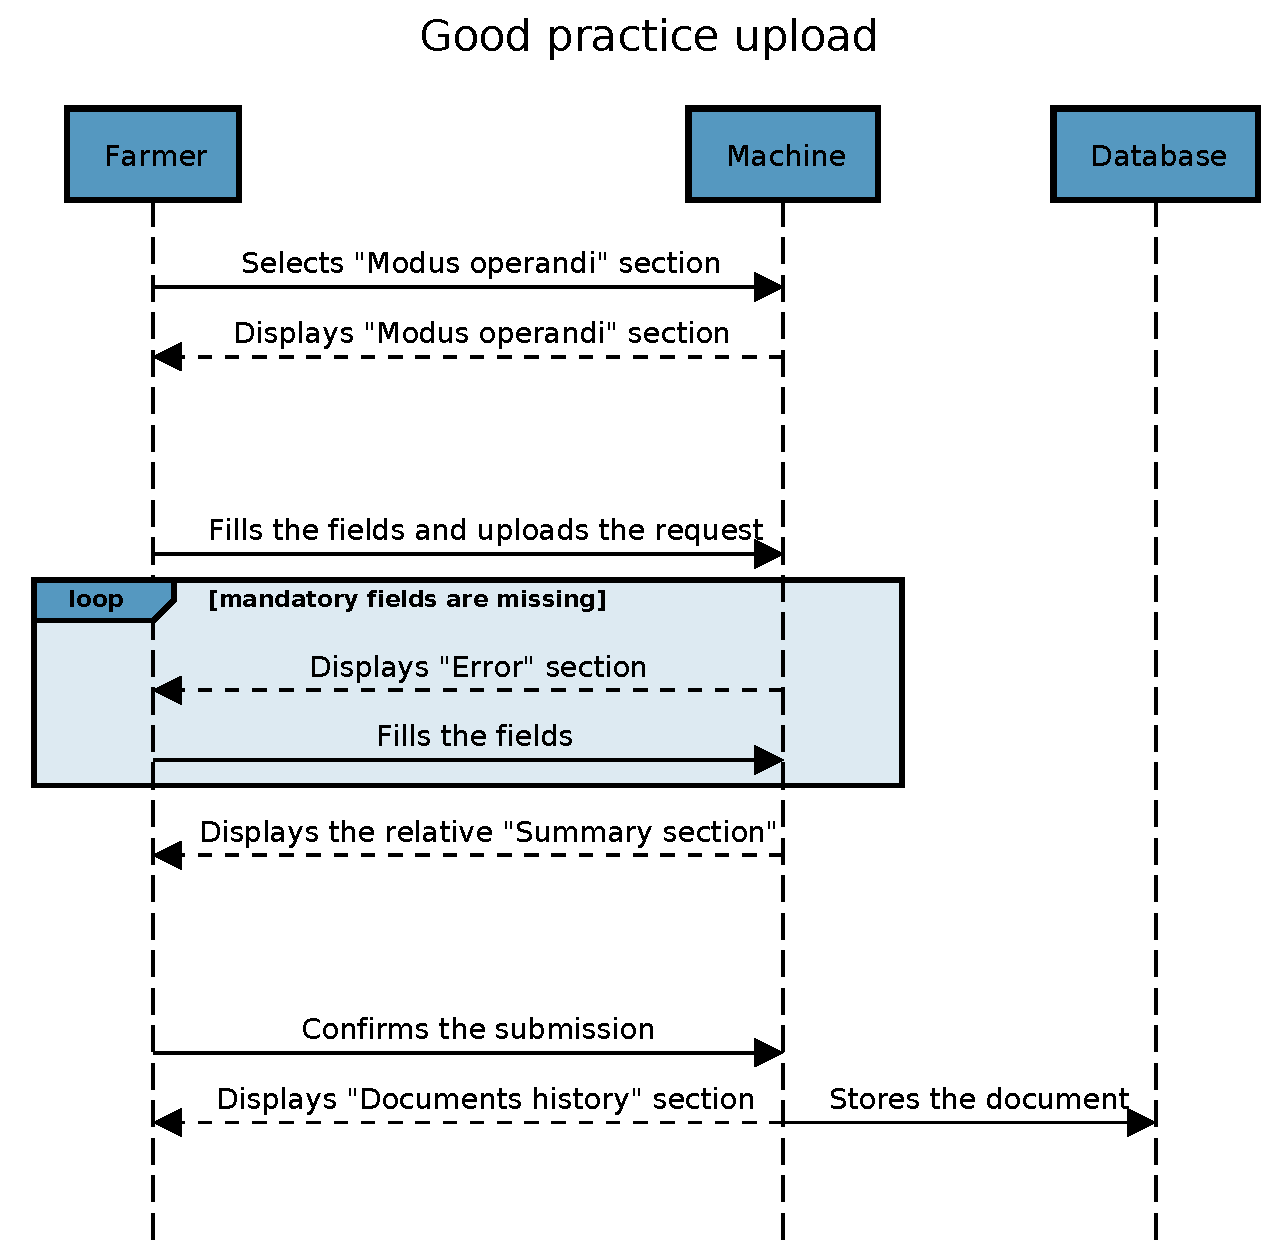
\includegraphics[page=1, width=\textwidth]{Images/SeqDiag/good_practice_seq_diag.pdf}
	\caption{\label{fig:good_practice_seq_diag}Good practices upload - sequence diagram}
\end{figure}


\begin{table}[H]
    \centering
    \begin{tabular}{|l|p{0.75\textwidth}|}
        \hline % ---------------------------------------------------------------------
    	\textsc{id}                 &   F.6\\
    	\hline % ---------------------------------------------------------------------
    	\textsc{Name}               &   Visualize relevant data\\
    	\hline % ---------------------------------------------------------------------
    	\textsc{Actor}             &   Farmer\\
    	\hline % ---------------------------------------------------------------------
    	\textsc{Entry condition}   &   Farmer has logged in\\
    	\hline % ---------------------------------------------------------------------
    	\textsc{Events flow}         &   %\footnotesize
            	                        \begin{itemize}
                                    	    \item Farmer selects the graphical section responsible for the relevant data visualization, called informally \textit{Relevant data section}
                                        \end{itemize}\\
        \hline % ---------------------------------------------------------------------
        \textsc{Exit condition}    &  The application displays a section containing information about weather forecasts, farm related tools suggestion, agronomist visit time, amount of water used that month, soil humidity etc.)\\
    	\hline % ---------------------------------------------------------------------
    	\textsc{Output}             &  \begin{itemize}
    	    \item The farmer can visualize relevant information
    	    \item Farmer can interact with information (links to shop websites etc.)
    	\end{itemize}\\
    	\hline % ---------------------------------------------------------------------
    	\textsc{Exception}         &   If the internet connection is lost, the application displays a section informing the task cannot be achieved\\
    	\hline % ---------------------------------------------------------------------
        
    \end{tabular}

\caption{\label{tab:visualize_relevant_data}Visualize relevant data for farmers}
\end{table}

\begin{figure}[H]
	\centering
    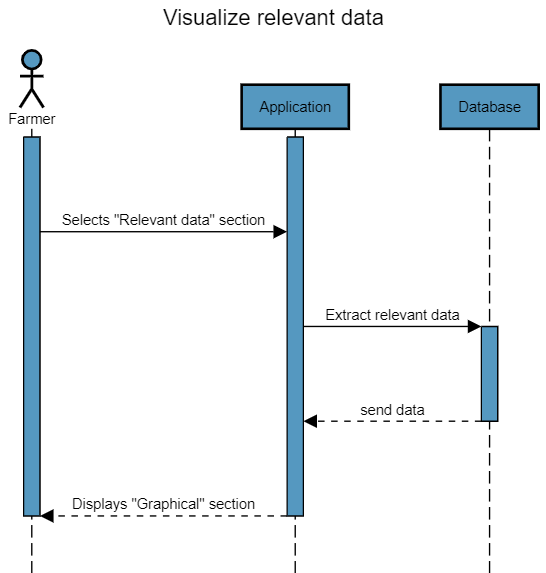
\includegraphics[page=1, width=\textwidth]{Images/Sequence diagrams/SW2 - Visualize relevant data (fa).png}
	\caption{\label{fig:good_practice_seq_diag} Visualize relevant data - sequence diagram}
\end{figure}

\subsubsection{Agronomists}
\label{sect:agronomist_requirements}
In this section there will be presented agronomists use case tables \ldots

% USE CASE TABLE 1: INSERT THE AREA AGRONOMISTS ARE RESPONSIBLE OF
\begin{table}[H]
    \centering
    \begin{tabular}[c]{|l|p{0.75\textwidth}|}
        \hline % ---------------------------------------------------------------------
    	\textsc{id}                 &   A.1\\
    	\hline % ---------------------------------------------------------------------

    	\textsc{Name}               &   Add an area under the agronomist's responsibility\\
    	\hline % ---------------------------------------------------------------------
    	\textsc{Actor}             &   Agronomist\\
    	\hline % ---------------------------------------------------------------------
    	\textsc{Entry condition}   &   Agronomist has logged in\\
    	\hline % ---------------------------------------------------------------------
    	\textsc{Events flow}         &   %\footnotesize
            	                        \begin{itemize}
                                    	    \item Agronomist goes to the "Area management" section
                                    	    \item The system extracts the data from the database and displays the list of areas under the agronomist's responsibility
                                    	    \item Agronomist presses the button “Add an area”
                                    		\item The system displays a page with all the available areas and a search bar
                                    		\item Agronomist makes a research based on the name/location of the area
                                    		\item The system shows the results
                                    		\item Agronomist selects the desired area
                                    		\item The system shows the details of the area selected (number of farmers, number of agronomists, weather information, etc)
                                    		\item Agronomist clicks on “Add this area”
                                    		\item The system updates the database and shows a message of insertion completed
                                        \end{itemize}\\
        \hline % ---------------------------------------------------------------------
        \textsc{Exit condition}    &  The system displays the "Area management" section\\
    	\hline % ---------------------------------------------------------------------
    	\textsc{Output}             &  \begin{itemize}
    	    \item The system has added the agronomist in the database as responsible for that area
    	\end{itemize}\\
    	\hline % ---------------------------------------------------------------------
    	\textsc{Exception}         &  Agronomist wrongly clicks “Add this area”. The system displays a popup notifying that he will be added as responsible for that area and the agronomist clicks on “Cancel” button\\
    	\hline % ---------------------------------------------------------------------
        
    \end{tabular}
    \caption{\label{tab:responsible_area_insertion}Add an area for an agronomist}
\end{table}

\begin{figure}[H]
    \centering
    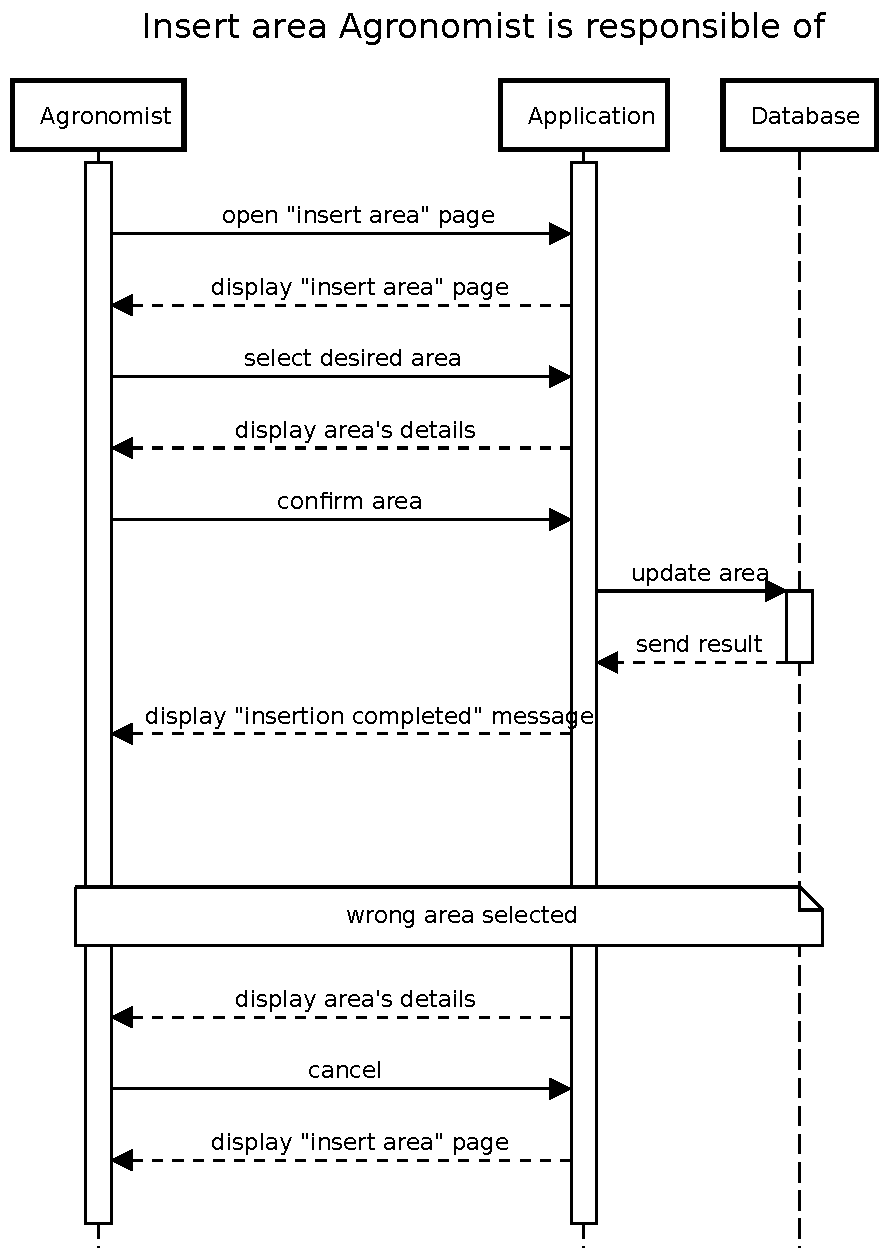
\includegraphics[scale=0.75]{Images/Sequence diagrams/Agronomist - Insert area.pdf}

    \caption{Add an area for an agronomist - sequence diagram}
    \label{fig:fig:seq_diag_insert_area}

    
\end{figure}


% USE CASE 2: REMOVING AN AREA UNDER THE AGRONOMIST'S RESPONSIBILITY
\begin{table}[H]
    \centering
    \begin{tabular}[c]{|l|p{0.75\textwidth}|}
        \hline % ---------------------------------------------------------------------
    	\textsc{id}                 &   A.2\\
    	\hline % ---------------------------------------------------------------------
    	\textsc{Name}               &   Remove an area under the agronomist's responsibility\\
    	\hline % ---------------------------------------------------------------------
    	\textsc{Actor}             &   Agronomist\\
    	\hline % ---------------------------------------------------------------------
    	\textsc{Entry conditions}   &  
    	\begin{itemize}
                                    	    \item Agronomist has logged in
                                    	    \item Agronomist is responsible for at least one area
                                        \end{itemize}\\
    	\hline % ---------------------------------------------------------------------
    	\textsc{Events flow}         &   %\footnotesize
            	                        \begin{itemize}
                                    	    \item Agronomist goes to the "Area management" section
                                    	    \item The system extracts the data from the database and displays the list of areas under the agronomist's responsibility
                                    	    \item Agronomist presses the button “Remove this area” next to the desired area
                                    		\item The system displays a popup asking for confirmation
                                    		\item Agronomist clicks on “Confirm”
                                    		\item The system updates the database and shows a message of removal completed
                                        \end{itemize}\\
        \hline % ---------------------------------------------------------------------
        \textsc{Exit condition}    &  The system displays the "Area management" section\\
    	\hline % ---------------------------------------------------------------------
    	\textsc{Output}             &  \begin{itemize}
    	    \item The system has removed the agronomist in the database as responsible for that area
    	\end{itemize}\\
    	\hline % ---------------------------------------------------------------------
    	\textsc{Exception}         &  Agronomist wrongly clicks “Remove this area”. The system displays a popup notifying that he will be removed as responsible for that area and the agronomist clicks on “Cancel” button\\
    	\hline % ---------------------------------------------------------------------
        
    \end{tabular}
    \caption{\label{tab:responsible_area_insertion}Remove an area for an agronomist}
\end{table}

% USE CASE TABLE 2: ACCESS THE "REQUEST FOR HELP" SECTION

\begin{table}[H]
    \centering
    \begin{tabular}[c]{|l|p{0.75\textwidth}|}
        \hline % ---------------------------------------------------------------------
    	\textsc{id}                 &   A.3\\
    	\hline % ---------------------------------------------------------------------
    	\textsc{Name}               &   Visualize and answer to requests for help\\
    	\hline % ---------------------------------------------------------------------
    	\textsc{Actor}             &   Agronomist\\
    	\hline % ---------------------------------------------------------------------
    	\textsc{Entry condition}   &   Agronomist has logged in\\
    	\hline % ---------------------------------------------------------------------
    	\textsc{Events flow}         &   %\footnotesize
            	                        \begin{itemize}
                                    	    \item Agronomist goes to the “Requests for help” section
                                    		\item The system extracts the data from the database and displays a search bar and the list of conversations (sorted by recent activity), marking the ones which contains new messages
                                    		\item Agronomist selects a conversation
                                    		\item The system displays all the messages contained in that conversation and a text box
                                    		\item Agronomist writes in the text box an answer to the request and clicks “Send”
                                    		\item The system adds the message to the database
                                        \end{itemize}\\
        \hline % ---------------------------------------------------------------------
        \textsc{Exit condition}    &  The system remains in the same page, refreshing its content\\
    	\hline % ---------------------------------------------------------------------
    	\textsc{Output}             &  \begin{itemize}
    	    \item The system adds the message to the database
    	    \item The system notifies the participants of that conversation about the new message
    	\end{itemize}\\
    	\hline % ---------------------------------------------------------------------
    	\textsc{Exception}         &  The system cannot connect to the database/server. The system displays an error message.\\
    	\hline % ---------------------------------------------------------------------
        
    \end{tabular}
    \caption{\label{tab:help_request_section_access}Visualize and answer to requests for help}
\end{table}

\begin{figure}[H]
    \centering
    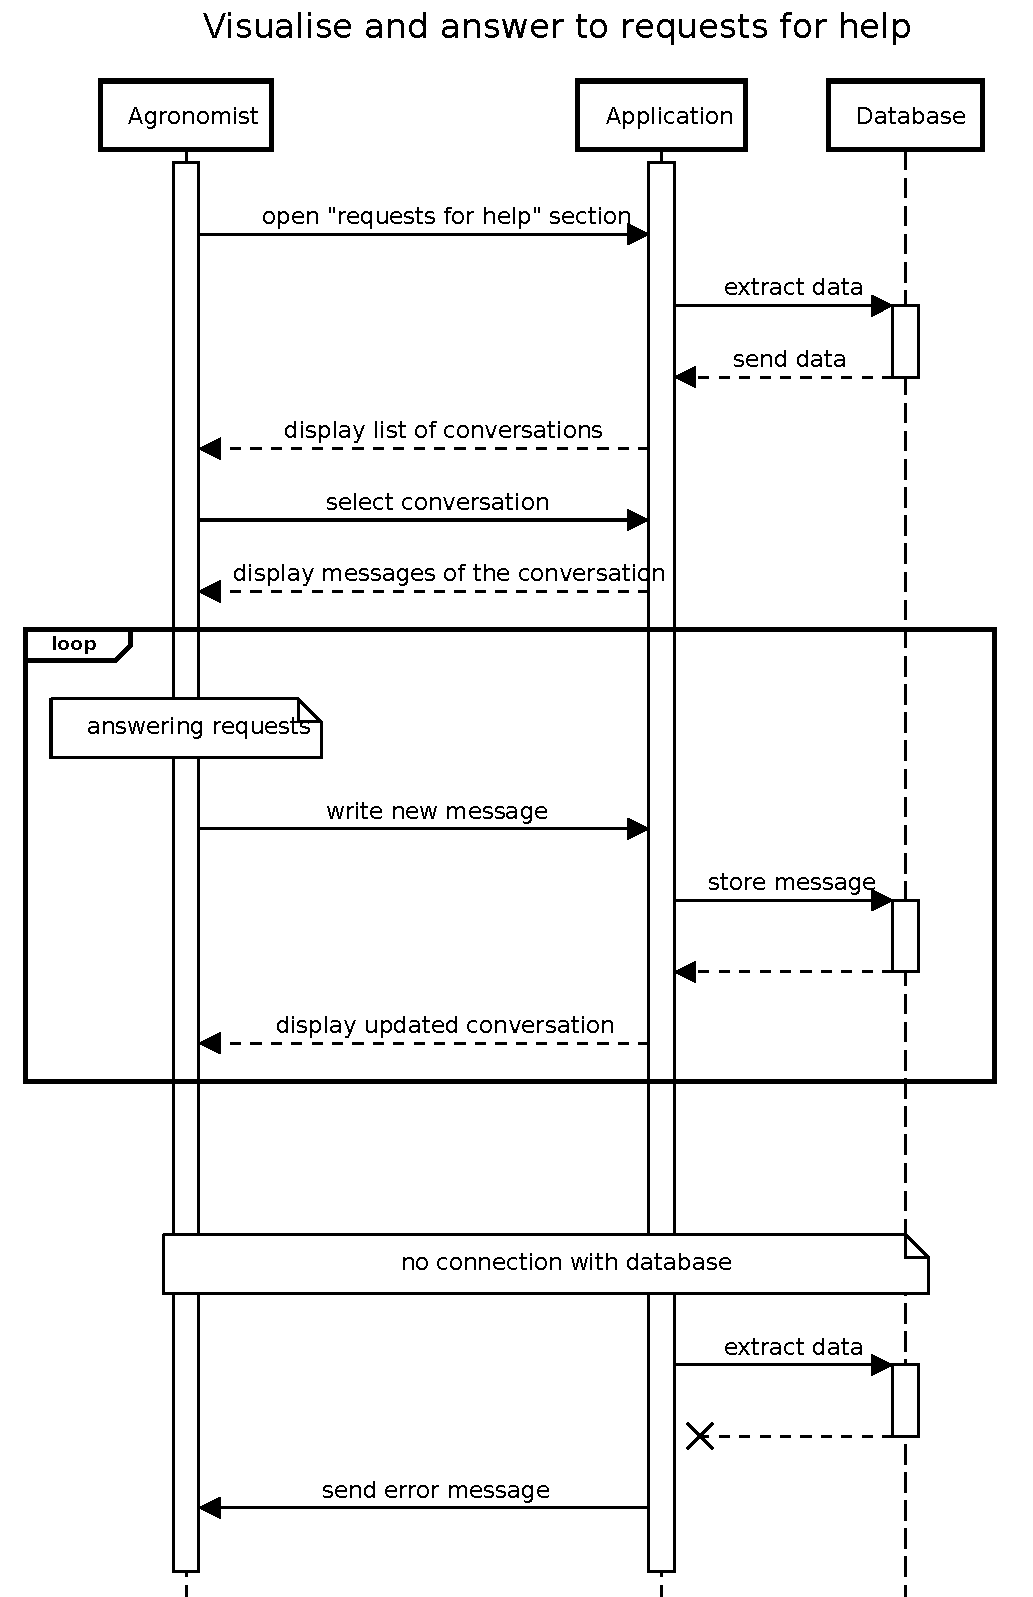
\includegraphics[scale=0.75]{Images/Sequence diagrams/Agronomist - visualise and answer requests for help.pdf}

    \caption{Visualize and answer to requests for help - sequence diagram}
    \label{fig:fig:seq_diag_answer_request}
\end{figure}

% USE CASE TABLE 3: VISUALIZE DATA OF THE AREA

\begin{table}[H]
    \centering
    \begin{tabular}[c]{|l|p{0.75\textwidth}|}
        \hline % ---------------------------------------------------------------------
    	\textsc{id}                 &   A.4\\
    	\hline % ---------------------------------------------------------------------
    	\textsc{Name}               &   Visualize data of an area\\
    	\hline % ---------------------------------------------------------------------
    	\textsc{Actor}             &   Agronomist\\
    	\hline % ---------------------------------------------------------------------
    	\textsc{Entry condition}   &   Agronomist has logged in\\
    	\hline % ---------------------------------------------------------------------
    	\textsc{Events flow}         &   %\footnotesize
            	                        \begin{itemize}

                                    	    \item Agronomist goes to the “Information about areas” section
                                    	    \item The system extract the data from the database and displays the list of areas under the agronomist's responsibility
                                    	    \item Agronomist selects an area
                                    		\item The system displays a page with three main options: “Weather forecasts”, “Farmers’ performing situation” and "Problems encountered"
                                    		\item Agronomist selects  the “Weather forecasts” section
                                    		\item The system extracts the data from the database and shows all the information concerning the weather forecasts in that area
                                    		\item Agronomist selects the “Farmers’ performing situation” section
                                    		\item The system extracts the data from the database and displays the list of all the farmers in the area, grouping them in “Best performing”, “Normal performing” and “Under-performing”
                                    		\item Agronomist selects a farmer
                                    		\item The system displays detailed information about that farmer (overall situation, planned visits, past visits, problems encountered)
                                    		\item Agronomist selects the "Problems encountered" section
                                    		\item The system displays the list of problems inserted by the farmers belonging to the Agronomist's area
                                        \end{itemize}\\
        \hline % ---------------------------------------------------------------------
        \textsc{Exit condition}    &  The system returns to the main page\\
    	\hline % ---------------------------------------------------------------------
    	\textsc{Exceptions}         &  The system cannot connect to the database/server. The system displays an error message.
    	\\
    	\hline % ---------------------------------------------------------------------
        
    \end{tabular}
    \caption{\label{tab:Area_information_access}Visualize data of an area}
\end{table}

\begin{figure}[H]
    \centering
    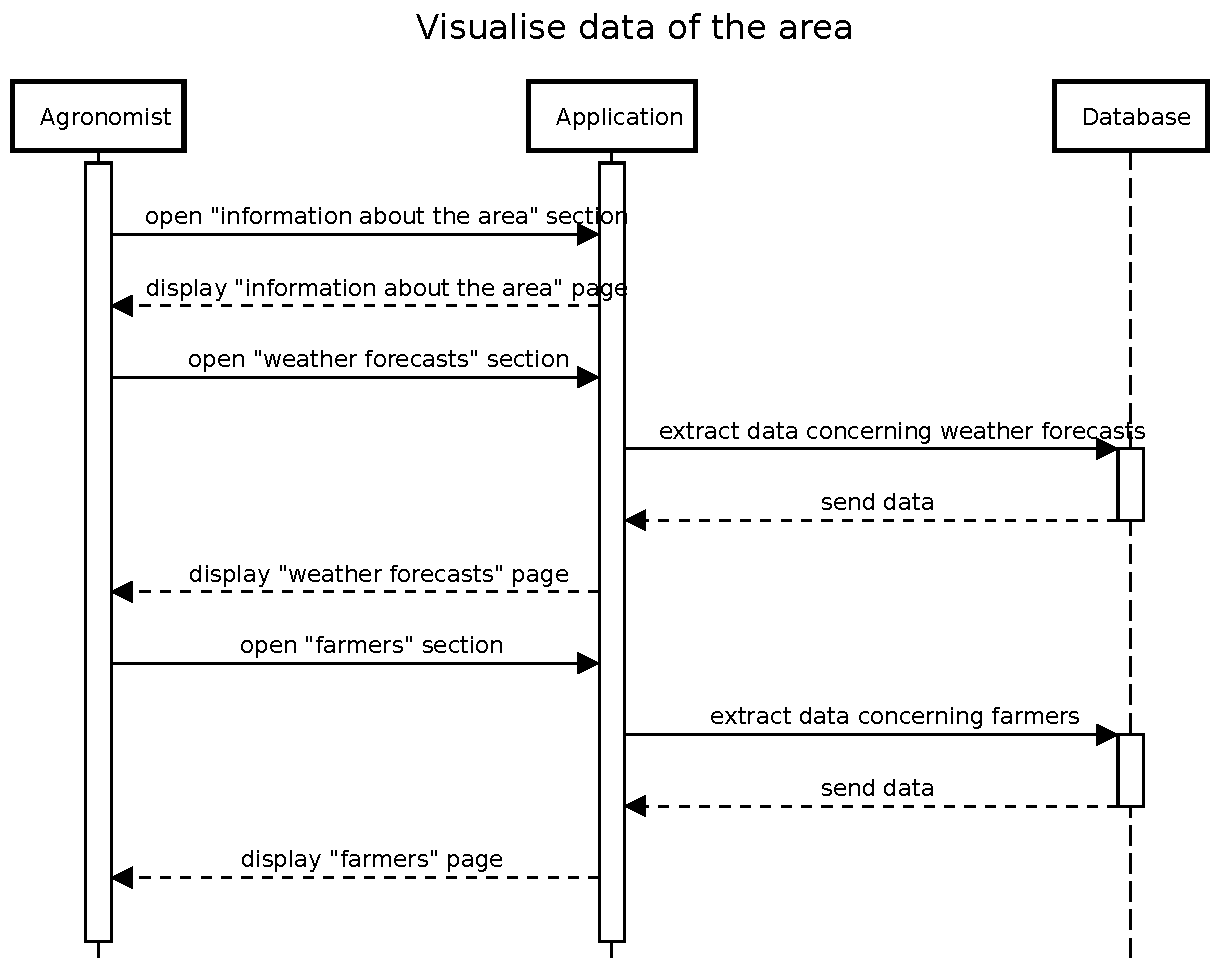
\includegraphics[scale=0.65]{Images/Sequence diagrams/Agronomist - visualise data of the area.pdf}

    \caption{Visualize data of an area - sequence diagram}
    \label{fig:fig:seq_diag_visualize_area}
\end{figure}

% USE CASE TABLE 4: ACCESS THE "DAILY PLAN" SECTION


\begin{table}[H]
    \centering
    \begin{tabular}[c]{|l|p{0.75\textwidth}|}
        \hline % ---------------------------------------------------------------------
    	\textsc{id}                 &   A.5\\
    	\hline % ---------------------------------------------------------------------
    	\textsc{Name}               &   Visualize and update a daily plan\\
    	\hline % ---------------------------------------------------------------------
    	\textsc{Actors}             &   Agronomist\\
    	\hline % ---------------------------------------------------------------------
    	\textsc{Entry conditions}   &   \begin{itemize}
                                    	    \item Agronomist has logged in
                                    	    \item At least one daily plan is present
                                        \end{itemize}\\
    	\hline % ---------------------------------------------------------------------
    	\textsc{Events flow}         &   %\footnotesize
            	                        \begin{itemize}
                                    	    \item Agronomist goes to the “Daily Plan” section, which is divided in “Visualize/Update” and “Confirm/Specify deviation from”. Agronomist selects the “Visualise/Update” section
                                    		\item The system extracts the data from the database and displays the list of daily plans for that agronomist
                                    		\item Agronomist selects a daily plan
                                    		\item The system displays all the information about that daily plan (day-month-year, farmers to be visited)
                                    		\item Agronomist clicks on the “Update” button
                                    		\item The system displays the list of farmers contained in the selected daily plan
                                    		\item Agronomist clicks on the “Remove” button near the farmer he wants to remove
                                            \item The systems displays the updated list of farmers
                                            \item Agronomist clicks on the “Add farmer” button
                                            \item The system displays the list of all the farmers for which the agronomist is responsible of and that are not already in the selected daily plan. In addition, for each farmer it is shown the list of problems encountered and the list of past and future visits (planned also by other agronomists) in a sort of compact calendar
                                            \item Agronomist selects a subset of farmers and clicks on “Add”
                                            \item The system displays the updated list of farmers
                                            \item Agronomist checks the info and clicks on “Confirm changes”

                                        \end{itemize}\\
        \hline % ---------------------------------------------------------------------
        \textsc{Exit condition}    &  The system shows a popup to notify the agronomist of the success of the operation
        \\
    	\hline % ---------------------------------------------------------------------
    	\textsc{Output}             &  \begin{itemize}
    	    \item The updated daily plan is stored in the database
    	\end{itemize}\\
    	\hline % ---------------------------------------------------------------------
    	\textsc{Exceptions}         &  \begin{itemize}
    	    \item The selected daily plan has already been confirmed and cannot be updated anymore. The system shows an error message.
    	    \item The selected daily plan is referring to the current day and cannot be updated anymore. The system shows an error message.
    	    \item Agronomist has made the wrong modifications to the daily plan. Instead of clicking “Confirm changes”, he/it clicks on “Discard changes”. The system displays the original daily plan and doesn’t store the new one in the database.    	\end{itemize}\\
    	
    	\hline % ---------------------------------------------------------------------
        
    \end{tabular}
    \caption{\label{tab:daily_plan_section_access}Visualize and update a daily plan}
\end{table}

\begin{figure}[H]
    \centering
    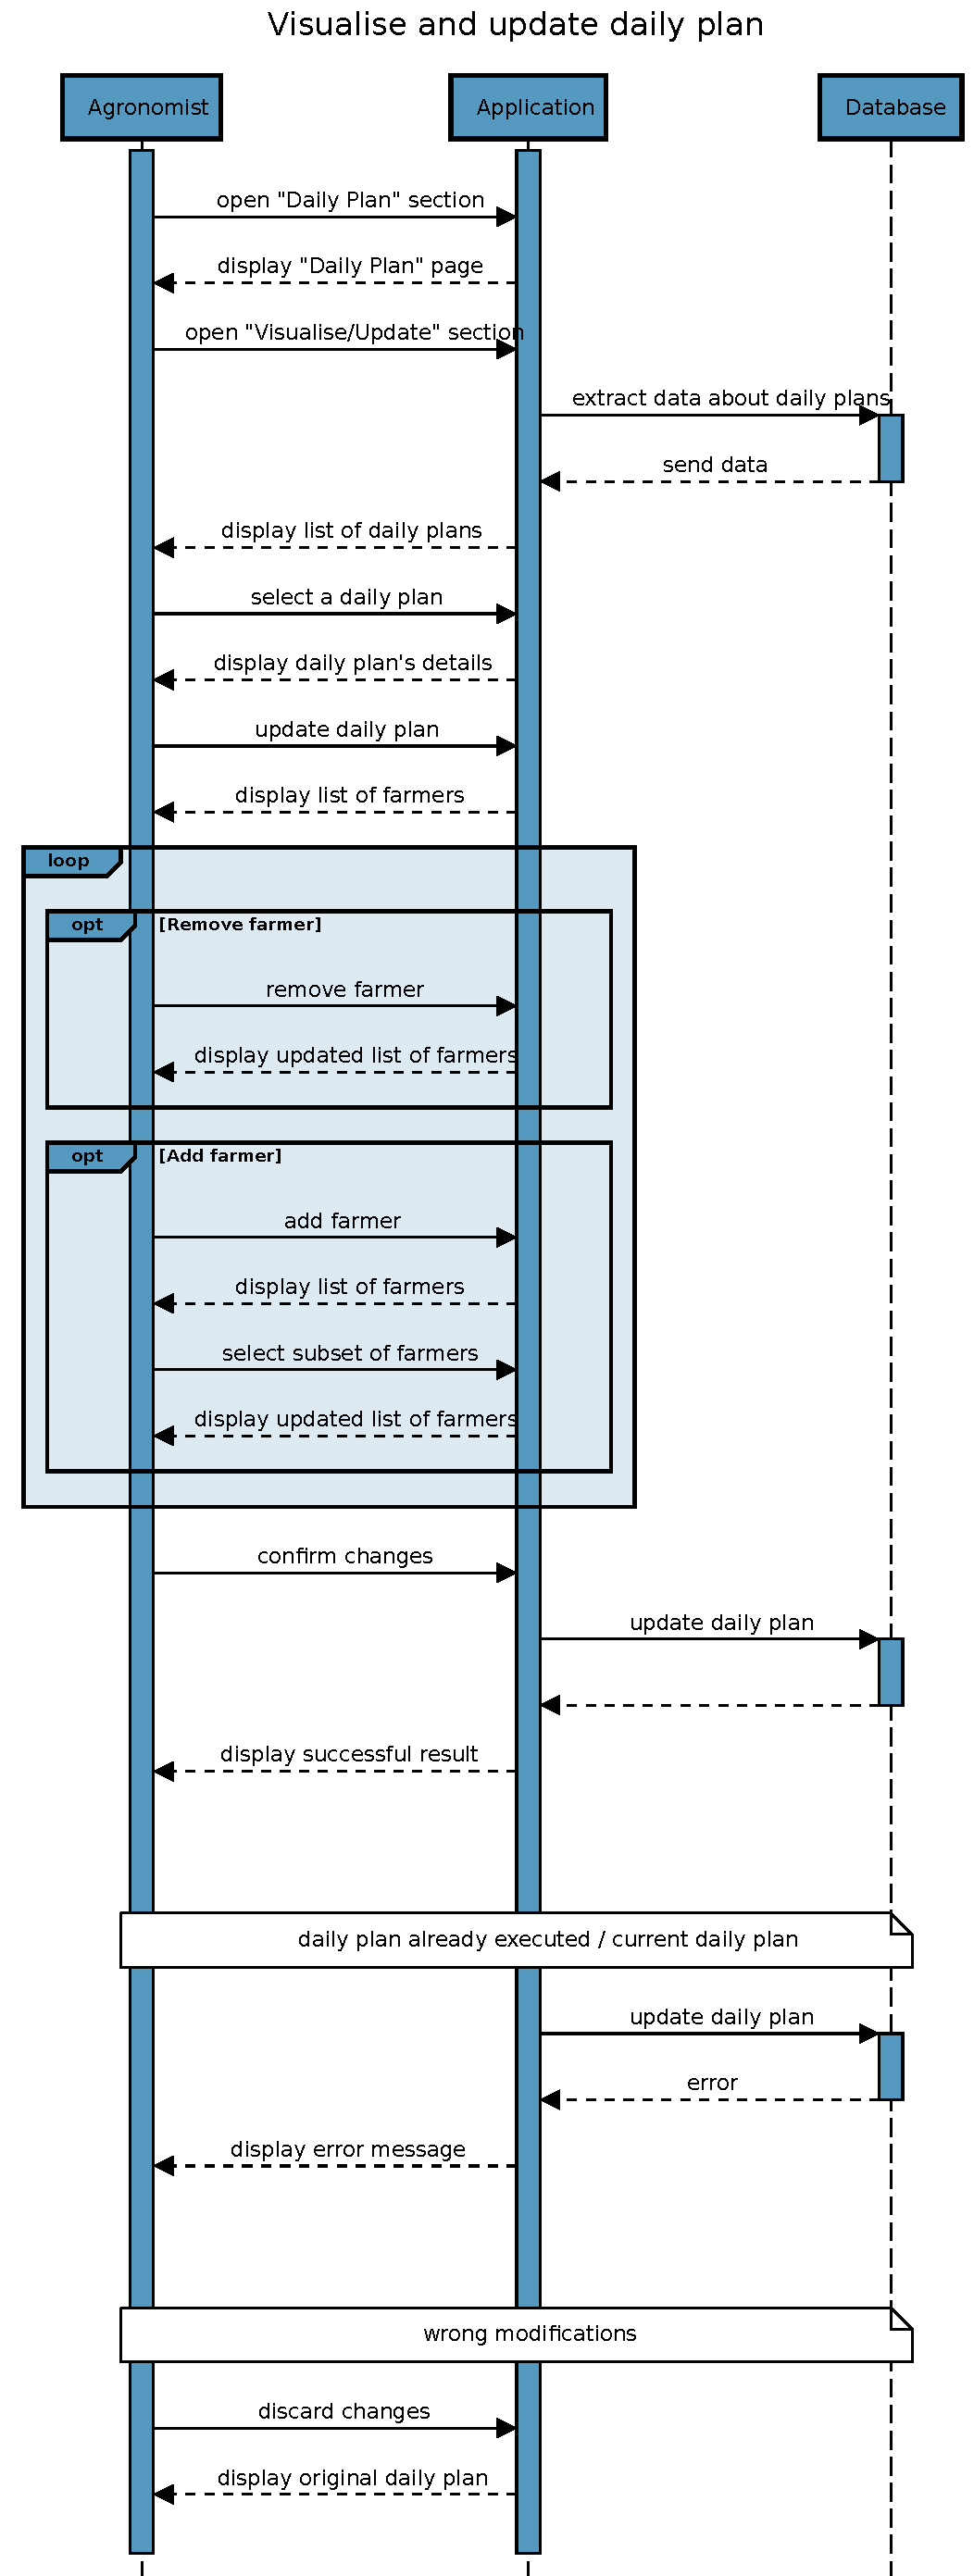
\includegraphics[scale=0.45]{Images/Sequence diagrams/Agronomist - visualise and update daily plan.pdf}

    \caption{Visualize and update a daily plan - sequence diagram}
    \label{fig:fig:seq_diag_update_daily_plan}
\end{figure}

% USE CASE TABLE 5: CONFIRM DEVIATIONS FROM DAILY PLAN


\begin{table}[H]
    \centering
    \begin{tabular}[c]{|l|p{0.75\textwidth}|}
        \hline % ---------------------------------------------------------------------
    	\textsc{id}                 &   A.6\\
    	\hline % ---------------------------------------------------------------------
    	\textsc{Name}               &   Confirm execution of daily plan\\
    	\hline % ---------------------------------------------------------------------
    	\textsc{Actor}             &   Agronomist\\
    	\hline % ---------------------------------------------------------------------
    	\textsc{Entry conditions}   &   \begin{itemize}
                                    	    \item Agronomist has logged in
                                    	    \item Agronomist has at least one daily plan
                                        \end{itemize}\\
    	\hline % ---------------------------------------------------------------------
    	\textsc{Events flow}         &   %\footnotesize
            	                        \begin{itemize}
                                    	    \item Agronomist goes to the “Daily Plan” section, which is divided in “Visualize/Update” and “Confirm/Specify deviation from”. Agronomist selects the “Confirm/Specify deviation from” section.
                                    		\item The system extracts the data from the database, displays the daily plan for the current day and enables the agronomist to select the subset of farmers which has not been visited that day
                                            \item Agronomist checks the info, selects the subset of farmers and clicks on “Continue”
                                            \item The system displays a compact summary of the info and asks for confirmation
                                            \item Agronomist checks the info and clicks on “Confirm”

                                        \end{itemize}\\
        \hline % ---------------------------------------------------------------------
        \textsc{Exit condition}    &  The system shows a popup to notify the agronomist of the success of the operation
        \\
    	\hline % ---------------------------------------------------------------------
    	\textsc{Output}             &  \begin{itemize}
    	    \item The system stores the completed daily plan in the database 
            \item The system increments by one the number of visits received by the farmers that actually have been visited
            \item The system rearranges the non-visited farmers in future daily plans

    	\end{itemize}\\
    	\hline % ---------------------------------------------------------------------
    	\textsc{Exception}         &  Agronomist has selected the wrong subset of farmers. Given the compact summary, it clicks on “Cancel”. The system displays again the daily plan and enables the agronomist to choose another subset of farmers.\\
    	
    	\hline % ---------------------------------------------------------------------
        
    \end{tabular}
    \caption{\label{tab:confirm_deviations_section}Confirm execution of daily plan}
\end{table}

\begin{figure}[H]
    \centering
    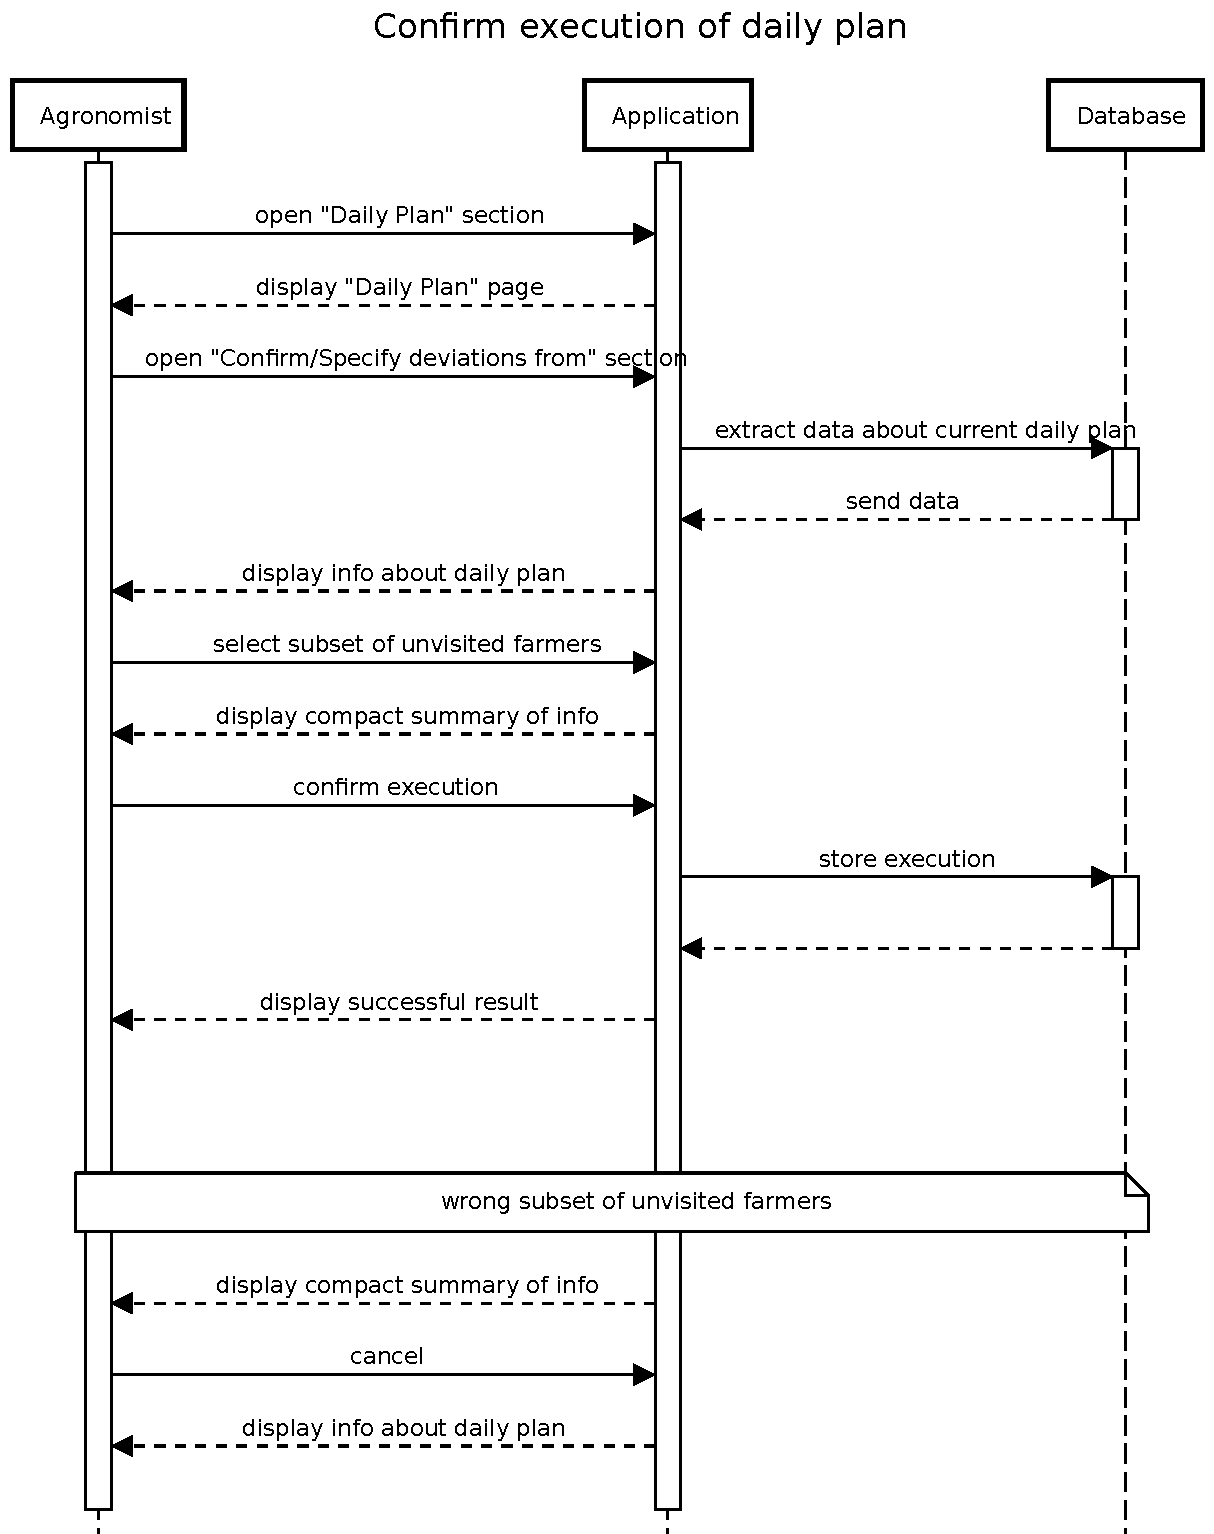
\includegraphics[scale=0.75]{Images/Sequence diagrams/Agronomist - confirm execution of daily plan.pdf}

    \caption{Confirm execution of daily plan - sequence diagram}
    \label{fig:fig:seq_diag_confirm_daily_plan}
\end{figure}



\subsection{Design Constraints}
\subsubsection{Standards compliance}
\subsubsection{Hardware limitations}

\subsection{Software System Attributes}
\subsubsection{Easy usability}
\subsubsection{Reliability}
\subsubsection{Availability}
\subsubsection{Security}
\subsubsection{Cross Platform}
\subsubsection{Modularity}
\subsubsection{Portability}

%------------------------------------------------------------------------------------------------------------------------------------------------
\clearpage
{\color{Blue}{\section{Formal Analysis Using Alloy}}}
\label{sect:alloy}
In this section we provide the whole \texttt{Alloy} code used for the analysis of the \hyperref[tab:acronymsTable]{S2B}, the results of the assertions and the diagrams representing the different worlds generated by the predicates.

\subsection{Alloy Code}
\alloyfile{Alloy/alloy code.als}

\newpage


\subsection{Assertions}

\begin{figure}[H]
    \centering
    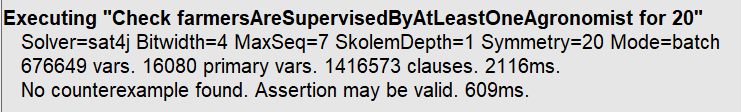
\includegraphics[]{Images/Alloy/assertion - farmersAreSupervisedByAtLeastOneAgronomist.png}
    \caption{Assertion 1}
    \label{fig:assertion1}
\end{figure}

\begin{figure}[H]
    \centering
    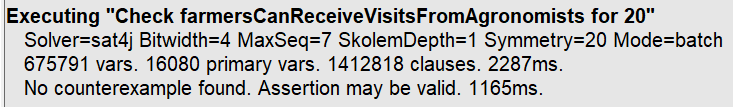
\includegraphics[]{Images/Alloy/assertion - farmersCanReceiveVisitsFromAgronomists.png}
    \caption{Assertion 2}
    \label{fig:assertion2}
\end{figure}

\begin{figure}[H]
    \centering
    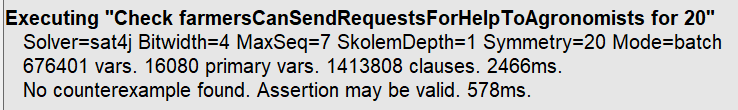
\includegraphics[]{Images/Alloy/assertion - farmersCanSendRequestsForHelpToAgronomists.png}
    \caption{Assertion 3}
    \label{fig:assertion3}
\end{figure}

\begin{figure}[H]
    \centering
    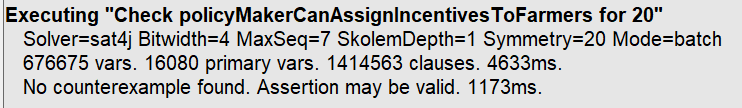
\includegraphics[]{Images/Alloy/assertion - policyMakerCanAssignIncentivesToFarmers.png}
    \caption{Assertion 4}
    \label{fig:assertion4}
\end{figure}

\newpage

\subsection{Worlds}

In this section we present the world diagrams generated by the Alloy predicates. This worlds are intended to show separate parts of the system, each one focusing on a different aspect.

\subsubsection*{World 1}
Figure \ref{fig:world1} represents a world focused on Daily Plans and Visits. It is possible to see that visits belonging to a specific daily plan have the same date of that daily plan. Also, a farmer cannot be visited twice in the same daily plan, while it is possible to receive visits in separate days. Moreover, it is possible to see that the farmers and the agronomist belong to the same area. In the end, each user has its own credentials.

\subsubsection*{World 2}
Figure \ref{fig:world2} represents a world focused on Requests, in this case a request for help. It is possible to see that each message sent in the "chat" is received by all the participants (except the sender, of course), while those users who do not belong to the "chat" (in this case Farmer1) cannot send or receive messages of that conversation. Also, a request has at least one agronomist as a participant (in this case even two). Moreover, the first message of the "chat" (ChatMessage2, isRequestMessage = True) is correctly sent by the farmer that made the request (Farmer0, startingUser), while the other messages are replies. In the end, each user has its own credentials.

\subsubsection*{World 3}
Figure \ref{fig:world3} represents a world focused on Forums. It is possible to see that different farmers can write (send a message) in the forum and each message is received by all farmers, while the agronomist does not participate to the forum. As for Requests (world 2), also here there is the correct mapping between the startingMessage (DiscussionMessage3) and the startingUser (Farmer0). In the end, each user has its own credentials.

\subsubsection*{World 4}
Figure \ref{fig:world4} represents a world focused on Good Practices. It is possible to see that each good practice has been requested by a policy maker and requested to a good-performing farmer. Also, the content of each practice is out of the scope of the analysis and is collapsed to a single entity (Text). Moreover, the agronomist does not act directly in this process. In the end, each user has its own credentials.

\subsubsection*{World 5}
Figure \ref{fig:world5} represents a world focused on Incentives. It is possible to see that a policy maker can assign incentives to a farmer (in this case different incentives to the same farmer) and there can be incentives not assigned yet (Incentive2). In this situation there are also two areas: each area has at least one agronomist (in this case the same one) and each farmer belongs to only one area. In the end, each user has its own credentials.

\newpage

\begin{figure}[H]
    \centering
    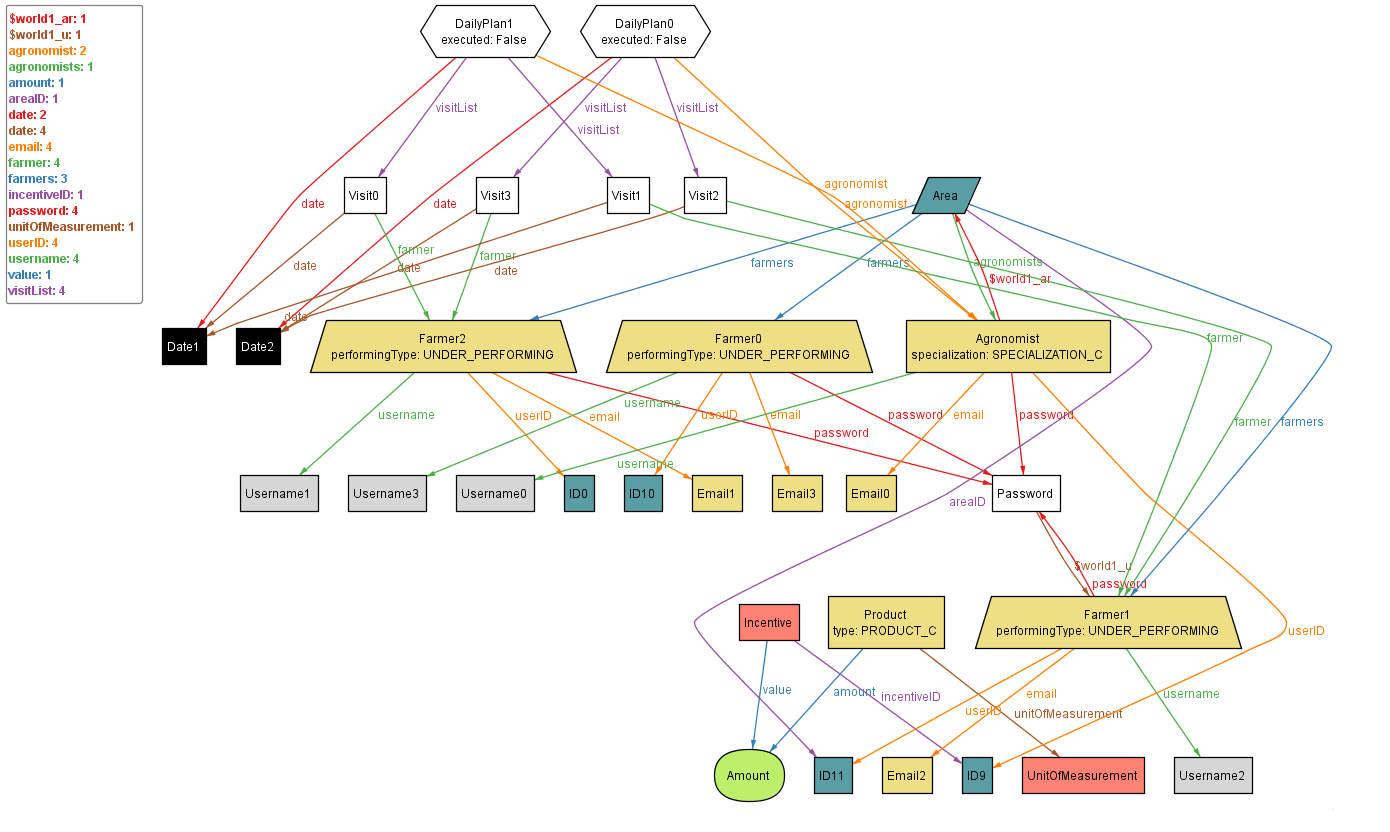
\includegraphics[angle=90, origin=c, width=0.85\textwidth]{Images/Alloy/world1.png}
    \caption{World focused on Daily Plans and Visits}
    \label{fig:world1}
\end{figure}

\begin{figure}[H]
    \centering
    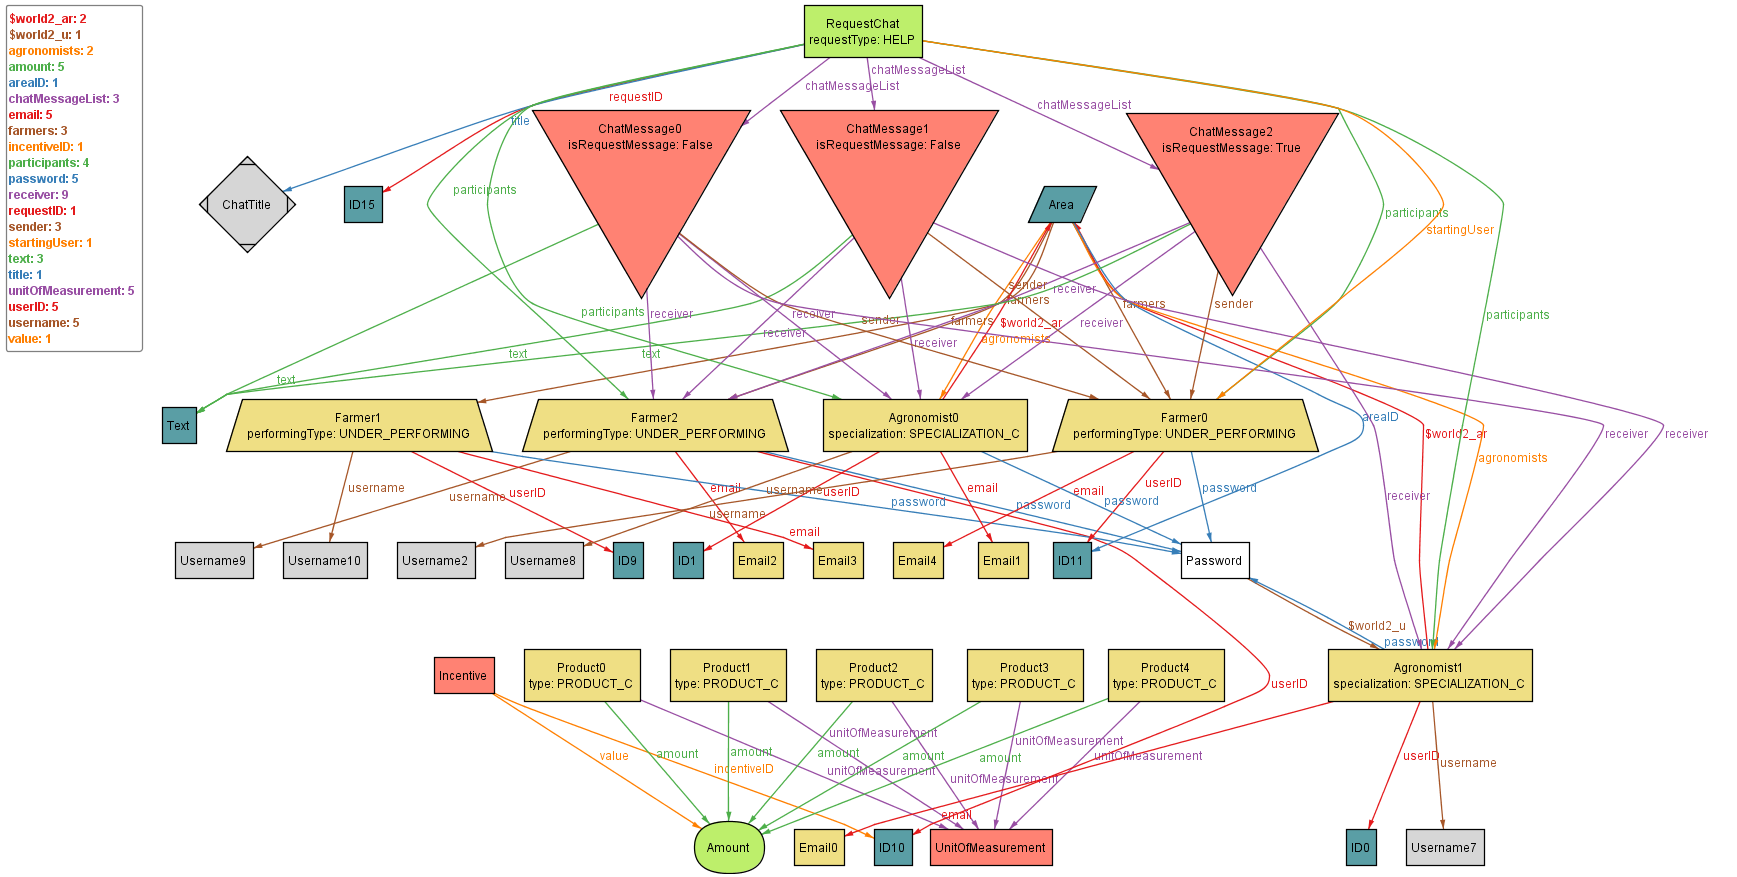
\includegraphics[angle=90, origin=c, width=0.75\textwidth]{Images/Alloy/world2.png}
    \caption{World focused on Requests}
    \label{fig:world2}
\end{figure}

\begin{figure}[H]
    \centering
    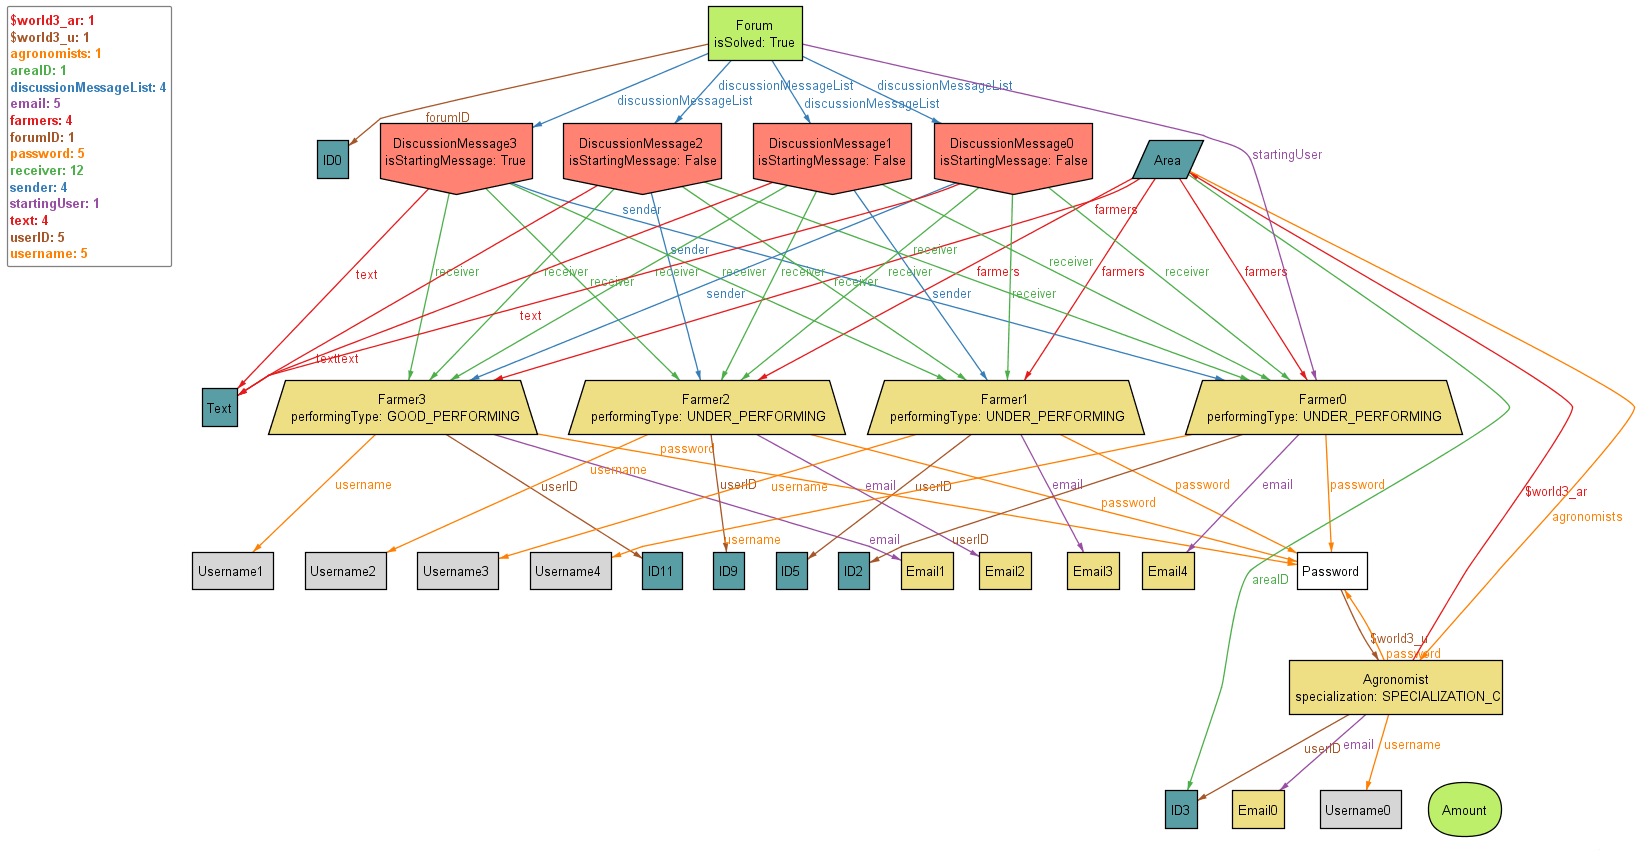
\includegraphics[angle=90, origin=c, width=0.75\textwidth]{Images/Alloy/world3.png}
    \caption{World focused on Forums}
    \label{fig:world3}
\end{figure}

\begin{figure}[H]
    \centering
    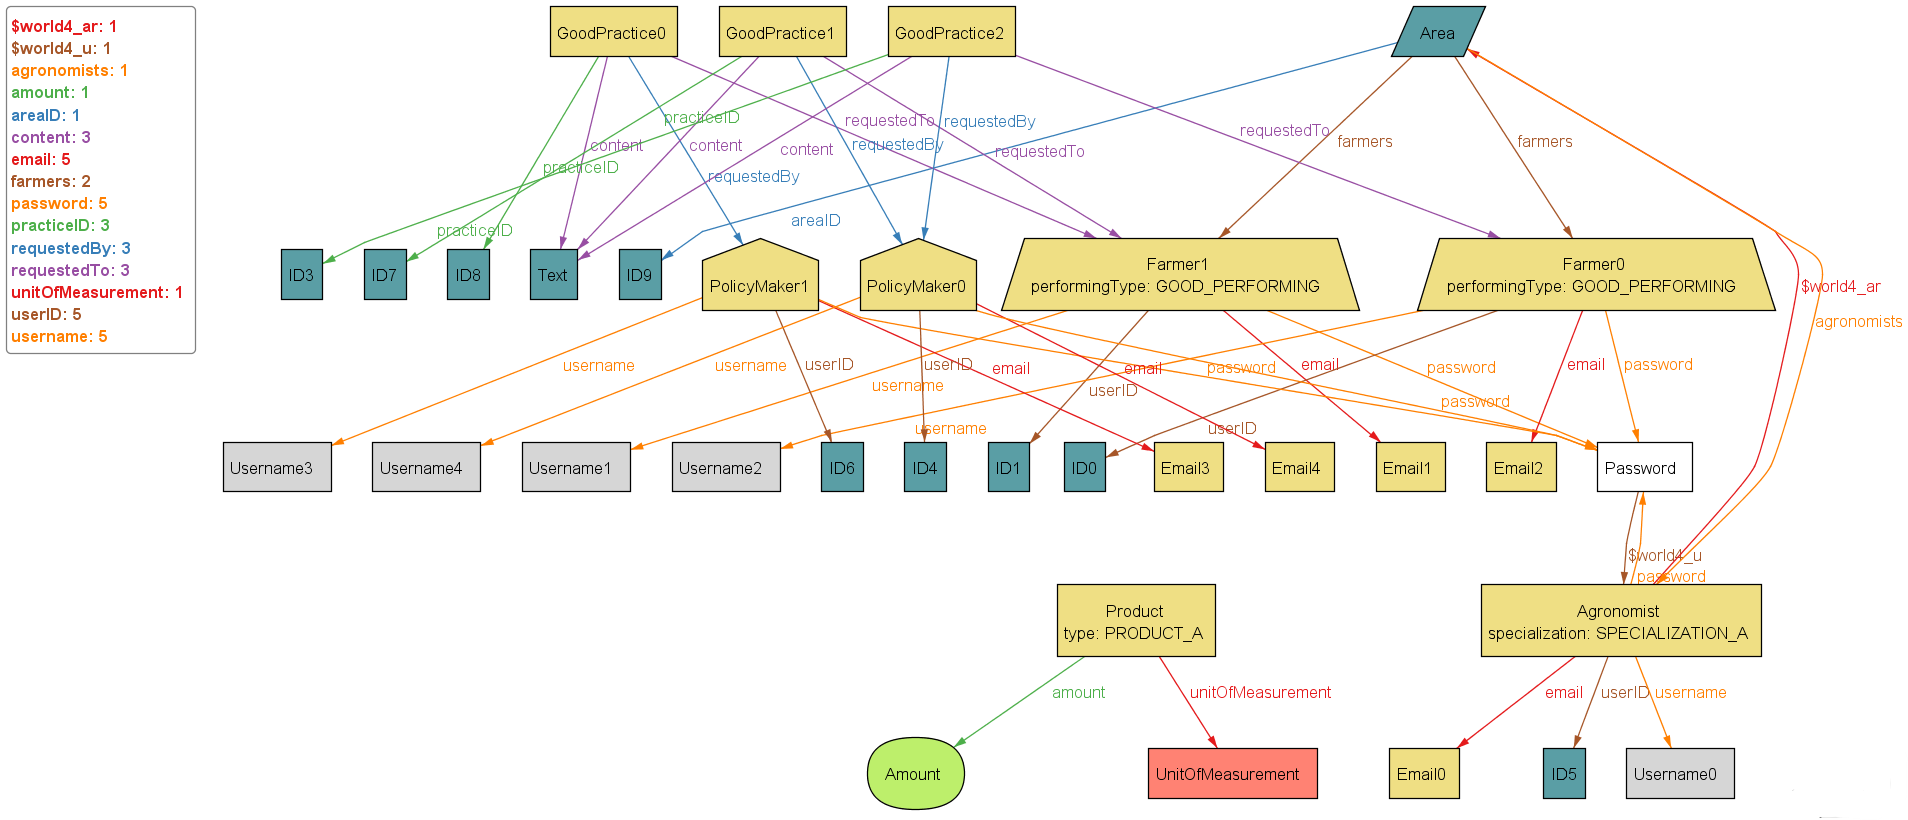
\includegraphics[angle=90, origin=c, width=0.6\textwidth]{Images/Alloy/world4.png}
    \caption{World focused on Good Practices}
    \label{fig:world4}
\end{figure}

\begin{figure}[H]
    \centering
    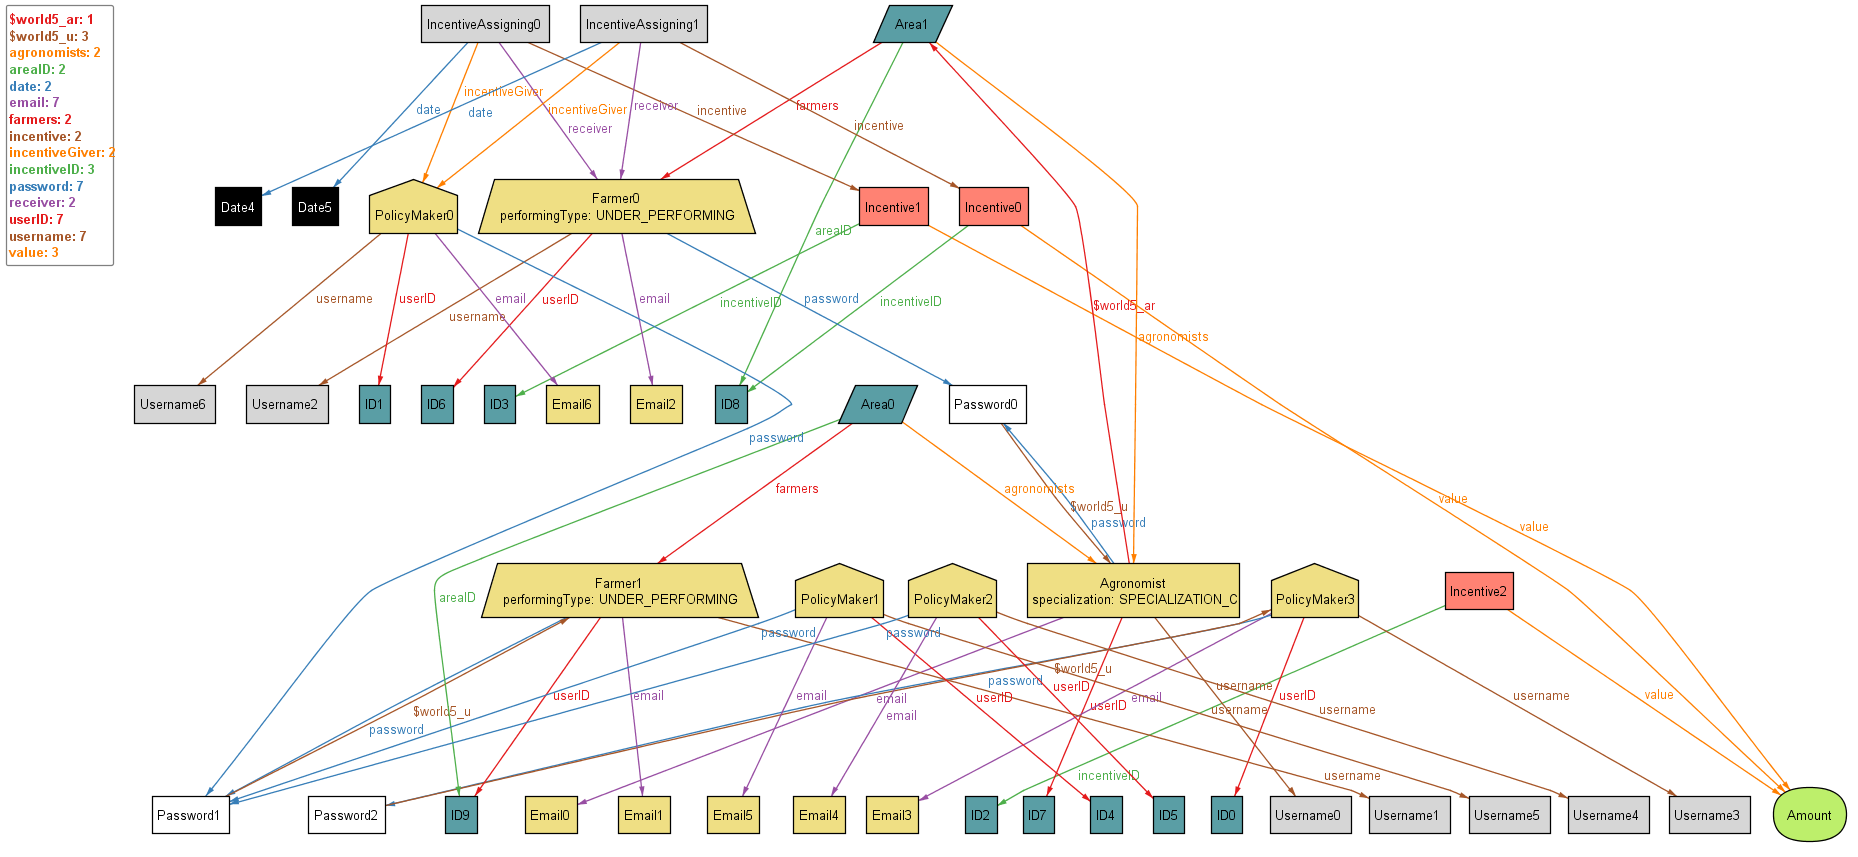
\includegraphics[angle=90, origin=c, width=0.65\textwidth]{Images/Alloy/world5.png}
    \caption{World focused on Incentives}
    \label{fig:world5}
\end{figure}

%------------------------------------------------------------------------------------------------------------------------------------------------
\clearpage
{\color{Blue}{\section{Effort Spent}}}
\label{sect:effort}
In this section we provide detailed information about how much effort each group member spent in working at this document. Further information about commits and updates is stored in the project \href{https://github.com/MarcoRomanini/GoriRomaniniWatanabe}{GitHub} repo. Furthermore also part of the Design Document effort is noted in the table below. 


\begin{center}
    \setlength\arrayrulewidth{1pt}
    \rowcolors{2}{myblue!25}{white}
    \begin{longtable}{llccc}
        
        \hline
        \rowcolor{myblue}\color{white}Date & \color{white}Description & \color{white}Gori & \color{white}Romanini & \color{white}Watanabe \\
        \hline
        29/10	&	World and Machine phenomena	&	2	&	2	&	2	\\
        \hline
        31/10	&	UML	&	1	&	1	&	1	\\
        \hline
        10/11	&	Goals, Domain assumptions, Requirements	&	3	&	3	&	3	\\
        \hline
        17/11	&	UML	&	4	&	4	&	4	\\
        \hline
        19/11	&	Functional requirements	&	4	&	4	&	4	\\
        \hline
        22/11	&	Actors	&		&	2	&		\\
        	&	Perspective (interfaces)	&	3	&		&		\\
        	&	Interface requirements	&		&		&	3	\\
        \hline
        24/11	&	Perspective (interfaces)	&	3	&		&		\\
        	&	Software system attributes	&		&	3	&		\\
        	&	Interface requirements	&		&		&	4	\\
        	&	Functional requirements	&	1	&	1	&		\\
        \hline
        26/11	&	Performance requirements	&		&	2	&		\\
        	&	Design constraints	&	3	&		&		\\
        	&	Functional requirements	&		&	2	&		\\
        	&	Product functions	&		&		&	4	\\
        	&	UI description	&		&		&	1	\\
        \hline
        29/11	&	Functional requirements	&		&	3	&		\\
        	&	farmer bpmn	&	3	&		&		\\
        \hline
        1/12	&	Alloy code	&		&	4	&		\\
        	&	farmer sequence diagram	&	3	&		&		\\
        	&	Users section introduction	&	1	&		&		\\
        \hline
        3/12	&	Goals, Domain assumptions, Requirements	&		&	1	&		\\
        	&	Alloy code	&		&	1,5	&		\\
        	&	Farmers goals mapping	&	2	&		&		\\
        \hline
        06/12	&	Alloy code	&		&	5	&		\\
        	&	UML	&		&	0,5	&		\\
        	&	UI description	&		&		&	3	\\
        	&	Goals, Domain assumptions, Requirements	&		&		&	4	\\
        	&	Introduction	&	6	&		&		\\
        \hline
        07/12	&	Functional Requirements (sequence diagrams, scenarios)	&		&	5	&		\\
        	&	UI design	&		&		&	5	\\
        	&	Sequence diagram	&		&		&	2	\\
        	&	bibliography	&	3	&		&		\\
        	&	latex edits, acronyms table	&	3	&		&		\\
        \hline
        10/12	&	UML diagram	&		&	1,5	&	1,5	\\
        	&	Functional Requirements (use cases)	&		&	1	&		\\
        	&	Product functions	&		&	2	&		\\
        	&	Farmers scenarios	&	3	&		&		\\
        	&	Use case diagram	&		&		&	2	\\
        	&	Policy maker scenarios	&		&		&	2	\\
        \hline
        13/12	&	Architecture Structure (Microservices)	&		&	3	&	3	\\
        \hline
        15/12	&	BPMN	&		&	0,5	&		\\
        	&	Alloy code	&		&	1	&		\\
        	&	Architecture Structure (Microservices)	&		&	1,5	&		\\
        	&	UML diagram	&		&		&	0,5	\\
        	&	BPMN	&		&		&	1	\\
        	&	Goals, Domain assumptions, Requirements	&		&		&	1	\\
        	&	Use case	&		&		&	1	\\
        	&	transcribed goals and requirements	&	1.5	&		&		\\
     	    &	transcribed domain assumptions and traceability matrix   	&	1.5	&		&		\\
        \hline
        17/12	&	UML description	&		&	1,5	&		\\
        	&	Added Alloy code with assertion	&	2	&		&		\\
        \hline
        20/12	&	Functional requirements	&		&	3,5	&		\\
        	&	Architecture Structure (Microservices)	&	1,5	&	1,5	&	1,5	\\
        	&	Alloy code	&		&	1	&		\\
        	&	UML diagram	&		&		&	1	\\
        	&	Goals, Domain assumptions, Requirements	&		&		&	1	\\
        	&	Sequence diagram	&		&		&	2	\\
        	&	Use cases	&		&		&	0,5	\\
        	&	Alloy code transcription	&	2	&		&		\\
        	&	Sequence diagram update	&	1	&		&		\\
        	&	Introduction revise	&	0.5	&		&		\\
        \hline
        20/12 & Effort table & 0.5 &    & \\
         & Whole document review & 7 & 7 & 7\\
        \hline
        
        \rowcolor{white}\caption{\label{tab:effort}Table of efforts.}
        
    \end{longtable}
\end{center}


%------------------------------------------------------------------------------------------------------------------------------------------------
\clearpage
\addcontentsline{toc}{section}{References}
\bibliographystyle{plain}
\bibliography{main}
%------------------------------------------------------------------------------------------------------------------------------------------------




\end{document}
